\section*{Introduction générale}
\addcontentsline{toc}{section}{Introduction générale}

Dans un environnement industriel exigeant en matière de productivité, de qualité et de disponibilité, la maintenance constitue une fonction stratégique. Une gestion efficace des opérations de maintenance contribue à réduire les arrêts non planifiés, à prolonger la durée de vie des équipements et à optimiser l’utilisation des ressources techniques et matérielles.

Toutefois, le recours à des documents papier, à des fichiers bureautiques et à des échanges d’informations non centralisés rend le suivi des équipements et des interventions plus complexe. La dispersion des données limite notamment l’accès aux historiques, la traçabilité des opérations et la visibilité sur l’état des machines, les pannes et les pièces consommées. Une gestion principalement corrective peut également entraîner des arrêts imprévus et une augmentation des délais d’intervention.

C’est dans ce contexte que s’inscrit ce projet de fin d’études, réalisé au sein d’IPROTEX Tunisie s.a.r.l. Il consiste à concevoir et à développer une plateforme web de Gestion de la Maintenance Assistée par Ordinateur (GMAO) destinée à centraliser les informations relatives aux machines, aux plans de maintenance, aux interventions, aux ordres de travail, aux documents techniques et aux pièces de rechange.

La plateforme distingue trois profils principaux : l’administrateur, l’opérateur et le technicien. Elle couvre la gestion des utilisateurs et des droits d’accès, des machines et de leurs modules, de la maintenance préventive et corrective, des ordres de travail, des stocks, des documents techniques, des notifications, des rapports et des indicateurs de performance.

Le projet intègre également la surveillance en temps réel des équipements à travers les protocoles MQTT et WebSocket ainsi qu’un service de détection d’anomalies appliqué aux données de roulements. Les résultats de cette analyse sont enregistrés et soumis à une validation humaine. Cette composante constitue une aide à la décision et ne remplace pas l’expertise des responsables de maintenance.

La problématique du projet peut ainsi être formulée comme suit :

\begin{quote}
\textit{Comment concevoir et développer une plateforme GMAO centralisée, sécurisée et évolutive permettant d’améliorer la gestion des équipements, la planification des opérations de maintenance, le suivi des interventions et l’exploitation des données techniques au sein d’IPROTEX Tunisie ?}
\end{quote}

Pour répondre à cette problématique, le projet vise principalement à centraliser les données de maintenance, à organiser les interventions préventives et correctives, à assurer la traçabilité des actions, à suivre les ordres de travail et les pièces de rechange, et à fournir des indicateurs adaptés aux responsabilités de chaque utilisateur.

Le développement a été conduit selon une démarche agile inspirée de Scrum. Le projet est organisé autour d’un Sprint 0 consacré à l’analyse et à la planification, suivi de sept Sprints de réalisation regroupant des ensembles fonctionnels cohérents.

Le présent rapport est organisé en neuf chapitres :

\begin{itemize}
    \item \textbf{Chapitre 1 -- Présentation générale :} présentation de l’organisme d’accueil, du projet, de l’étude préalable, de la solution proposée et de la méthodologie adoptée ;

    \item \textbf{Chapitre 2 -- Analyse et spécification des besoins :} identification des acteurs et des besoins, présentation du Product Backlog, planification des Sprints et description de l’architecture générale ;

    \item \textbf{Chapitre 3 -- Sprint 1 : Authentification et gestion des accès :} gestion de l’authentification, des utilisateurs, des profils, des rôles et des autorisations ;

    \item \textbf{Chapitre 4 -- Sprint 2 : Gestion des machines et des équipements :} gestion des machines, des modules et des documents techniques associés ;

    \item \textbf{Chapitre 5 -- Sprint 3 : Maintenance préventive :} gestion des plans, des listes de contrôle et du cycle de validation des interventions préventives ;

    \item \textbf{Chapitre 6 -- Sprint 4 : Maintenance corrective et ordres de travail :} signalement des pannes, gestion des interventions et suivi du cycle de vie des ordres de travail ;

    \item \textbf{Chapitre 7 -- Sprint 5 : Gestion des stocks, rapports et tableaux de bord :} suivi des pièces de rechange, des mouvements de stock, des notifications, des rapports et des indicateurs ;

    \item \textbf{Chapitre 8 -- Sprint 6 : Surveillance et maintenance prédictive :} supervision des équipements connectés, analyse des données et détection d’anomalies ;

    \item \textbf{Chapitre 9 -- Sprint 7 : Déploiement, supervision et DevSecOps :} automatisation des contrôles, déploiement, surveillance et sécurisation de la plateforme.
\end{itemize}

Enfin, la conclusion générale synthétise les résultats obtenus, les difficultés rencontrées, les apports du projet et ses perspectives d’évolution.


\newpage 

\section{Présentation Générale}
 
\subsection{Introduction}

Ce premier chapitre présente le cadre général du projet de fin d’études réalisé au sein d’IPROTEX Tunisie s.a.r.l. Il introduit l’organisme d’accueil, le contexte industriel, la problématique et les objectifs ayant conduit au développement de la plateforme GMAO.

Il expose ensuite les pratiques actuelles de maintenance ainsi qu’une étude comparative de solutions disponibles à l’échelle nationale et internationale. Cette analyse permet de dégager leurs principaux avantages et leurs limites par rapport aux besoins d’IPROTEX Tunisie, puis de justifier la solution proposée.

Enfin, ce chapitre présente la méthodologie agile adoptée et son adaptation à l’organisation du projet.

\subsection{Cadre général du stage}

Dans le cadre de ma formation d’ingénieur à l’École Supérieure Privée d’Ingénierie et de Technologies (ESPRIT), j’ai réalisé mon projet de fin d’études au sein d’IPROTEX Tunisie s.a.r.l., du 1\textsuperscript{er} mars au 1\textsuperscript{er} septembre 2026, sous l’encadrement de Monsieur Mohamed Yassine Den Debba.

Ce stage constitue une mise en application des connaissances techniques et méthodologiques acquises au cours de ma formation. Il m’a permis de participer aux différentes phases d’un projet informatique, depuis l’analyse des besoins jusqu’au déploiement, en passant par la conception, le développement et la validation.

La mission confiée consiste à concevoir et à développer une plateforme web de Gestion de la Maintenance Assistée par Ordinateur adaptée aux activités d’IPROTEX Tunisie. La solution vise à centraliser les informations de maintenance, à améliorer le suivi des équipements et à organiser les interventions réalisées par les opérateurs, les techniciens et les administrateurs.

Le périmètre du projet couvre notamment la gestion des utilisateurs, des machines, des documents techniques, des opérations préventives et correctives, des ordres de travail, des stocks et des indicateurs de maintenance. Il comprend également la surveillance des équipements, la détection d’anomalies et la mise en place d’une démarche DevSecOps pour contrôler la qualité, la sécurité, le déploiement et la supervision de la plateforme.

\subsection{Présentation de l’organisme d’accueil}

\subsubsection{IPROTEX Tunisie s.a.r.l. et le groupe IPROTEX}

IPROTEX Tunisie s.a.r.l. est l’implantation tunisienne du groupe allemand IPROTEX GmbH \& Co. KG. Fondé en 1999 et établi à Münchberg, en Allemagne, le groupe est spécialisé dans le développement et la fabrication de textiles techniques destinés à la protection de composants industriels \cite{iprotex_company}.

Les produits développés par IPROTEX sont notamment utilisés pour protéger les câbles, les faisceaux électriques, les tuyaux et d’autres composants contre la chaleur, l’abrasion, les vibrations et différentes contraintes mécaniques. L’industrie automobile constitue son principal secteur d’activité, mais le groupe intervient également dans les domaines ferroviaire, aéronautique, industriel et dans celui de la mobilité électrique \cite{iprotex_automotive}.

Le groupe dispose de plusieurs implantations internationales, notamment en Allemagne, en Tunisie, en Chine, au Mexique et en Macédoine du Nord. Cette présence lui permet d’accompagner ses clients et d’adapter ses solutions aux exigences de différents marchés industriels \cite{iprotex_environmental}.

Le présent projet de fin d’études est réalisé au sein d’IPROTEX Tunisie. Il s’inscrit dans un environnement de production où la disponibilité des machines et la bonne organisation des interventions de maintenance sont indispensables à la continuité des activités et au respect des exigences de qualité.

\begin{figure}[H]
    \centering
    
\includegraphics[width=0.25\textwidth]{figures/iprotex-Logo.png}
    \caption{Logo du groupe IPROTEX}
    \label{fig:logo-iprotex}
    
    \small Source : site officiel d’IPROTEX \cite{iprotex_company}.
\end{figure}

\subsubsection{Activités d’IPROTEX Tunisie s.a.r.l.}

IPROTEX développe et fabrique des solutions textiles adaptées aux contraintes thermiques, mécaniques et acoustiques rencontrées dans différents secteurs industriels. L’entreprise accompagne ses clients depuis l’analyse du besoin et la conception du produit jusqu’à sa fabrication en série.

Ses principales activités peuvent être résumées comme suit :

\begin{itemize}
    \item la recherche et le développement de textiles techniques ;
    \item la conception de solutions textiles personnalisées ;
    \item la fabrication de protections pour les câbles, les faisceaux électriques, les tuyaux et d’autres composants industriels ;
    \item le conseil technique et l’accompagnement des clients ;
    \item le contrôle de la qualité des produits fabriqués.
\end{itemize}

Pour fabriquer ces produits, le groupe utilise différents procédés, notamment le tressage, le tissage, le tricotage, le laminage, l’enduction et la découpe. La combinaison de ces procédés permet d’obtenir des solutions adaptées aux caractéristiques et aux contraintes de chaque application \cite{iprotex_tailormade}.

Le fonctionnement continu des équipements associés à ces procédés constitue un enjeu important pour IPROTEX Tunisie. Une panne ou une intervention mal planifiée peut affecter la continuité de la production et la qualité des produits. Ce contexte justifie la mise en place de la plateforme GMAO développée dans le cadre de ce projet, afin d’améliorer le suivi des machines et l’organisation des opérations de maintenance.


\subsection{Présentation du projet}

Le projet consiste à concevoir et à développer une plateforme web de Gestion de la Maintenance Assistée par Ordinateur adaptée aux activités d’IPROTEX Tunisie. Cette plateforme centralise les informations relatives aux équipements et assure l’organisation, l’exécution et le suivi des opérations de maintenance.

La solution couvre la gestion des utilisateurs, des machines et de leurs modules, des documents techniques, des plans de maintenance préventive, des interventions correctives, des ordres de travail et des pièces de rechange. Elle intègre également le suivi des stocks, les notifications, les rapports et les tableaux de bord.

La plateforme prend en charge trois profils principaux : l’administrateur, l’opérateur et le technicien. Une gestion des autorisations fondée sur les rôles permet à chaque utilisateur d’accéder uniquement aux données et aux fonctionnalités correspondant à ses responsabilités.

Le projet comporte également un mécanisme de surveillance en temps réel reposant sur la réception de données provenant d’équipements connectés. Un service indépendant de détection d’anomalies analyse certaines données techniques et soumet ses résultats à la validation des administrateurs ou des techniciens. Cette fonctionnalité constitue une aide à la décision et ne remplace pas l’expertise humaine.

\subsubsection{Objectif général du projet}

L’objectif principal du projet est de mettre à la disposition d’IPROTEX Tunisie une plateforme GMAO centralisée, sécurisée et évolutive permettant d’améliorer l’organisation des activités de maintenance.

Plus précisément, la solution vise à :

\begin{itemize}
    \item centraliser les informations relatives aux machines, aux interventions et aux documents techniques ;
    \item planifier et suivre les opérations de maintenance préventive ;
    \item gérer les pannes, les interventions correctives et les ordres de travail ;
    \item assurer le suivi des pièces de rechange et des mouvements de stock ;
    \item garantir la traçabilité des actions et des historiques de maintenance ;
    \item fournir des notifications, des rapports et des indicateurs d’aide à la décision ;
    \item exploiter les données des équipements connectés pour améliorer leur surveillance.
\end{itemize}

\subsubsection{Problématique}

IPROTEX Tunisie dispose de procédures et de référentiels permettant d’organiser ses activités de maintenance. Toutefois, les informations correspondantes sont réparties entre différents documents et fichiers, ce qui rend leur mise à jour, leur consultation et leur exploitation plus complexes.

Cette dispersion limite notamment la liaison entre les machines, les pannes, les interventions, les ordres de travail et les pièces consommées. Elle complique également la consultation des historiques, le suivi de l’avancement des interventions et la production d’indicateurs fiables.

La problématique principale du projet est donc formulée comme suit :

\begin{quote}
\textit{Comment concevoir et développer une plateforme GMAO centralisée, sécurisée et évolutive permettant d’améliorer la gestion des équipements, la planification des opérations de maintenance, le suivi des interventions et l’exploitation des données techniques au sein d’IPROTEX Tunisie ?}
\end{quote}

Pour répondre à cette problématique, la solution doit intégrer les référentiels existants, structurer les processus préventifs et correctifs, appliquer une gestion sécurisée des accès et assurer la traçabilité des opérations. Son architecture doit également permettre l’intégration progressive de nouvelles fonctionnalités selon les besoins de l’entreprise.


\subsection{Étude préalable}

Avant de concevoir la plateforme, une étude préalable a été menée afin d’analyser les pratiques de maintenance d’IPROTEX Tunisie et d’identifier les besoins auxquels la solution doit répondre.

Cette étude porte d’abord sur les procédures et les documents internes utilisés par l’entreprise. Elle est ensuite complétée par l’analyse de plusieurs solutions de GMAO disponibles à l’échelle nationale et internationale. Les résultats obtenus permettent d’identifier les limites de l’existant et de justifier la conception d’une solution adaptée au contexte de l’entreprise.

\subsubsection{Étude de l’existant}

\paragraph{Analyse des pratiques actuelles}

L’analyse des pratiques de maintenance d’IPROTEX Tunisie s’appuie sur les observations réalisées durant le stage et sur l’étude des documents internes mis à disposition. Ces documents comprennent notamment les plans de maintenance préventive relatifs aux processus de tressage, de découpe, d’enroulage et de bobinage \cite{braiding_maintenance,cutting_maintenance,rolling_maintenance,winding_maintenance}.

Ces plans définissent les équipements concernés, les opérations à réaliser, les responsables, les fréquences d’exécution et les méthodes de documentation. Ils couvrent principalement des tâches de contrôle, de nettoyage, de lubrification, de graissage et de remplacement périodique de certains composants.

Les plans étudiés montrent que l’entreprise dispose déjà de procédures préventives structurées :

\begin{itemize}
    \item le plan de tressage couvre notamment les fuseaux, les guides de fil, les capteurs, les mécanismes de tirage et les boîtes d’engrenages ;
    \item le plan de découpe concerne notamment les lames, les rouleaux de guidage, les dispositifs pneumatiques, les capteurs et les équipements de sécurité ;
    \item le plan d’enroulage comprend le contrôle des dispositifs pneumatiques, des articulations, des roulements, des filtres et des capteurs ;
    \item le plan de bobinage porte notamment sur les guides, les freins de fil, les courroies, les systèmes pneumatiques, les dispositifs de ventilation et les niveaux d’huile.
\end{itemize}

Les opérations détaillées, leurs fréquences et les illustrations correspondantes seront exploitées dans le Sprint consacré à la maintenance préventive. Les documents complets peuvent être placés en annexe afin de ne pas alourdir le corps du rapport.

L’entreprise dispose également d’un référentiel codifié des pannes, d’une liste des machines industrielles et de listes de pièces de rechange. Le référentiel des pannes associe les défaillances à des codes et à des informations utiles au suivi de la maintenance corrective et au calcul du temps moyen de réparation. La liste des machines contient les principales caractéristiques des équipements, tandis que les fichiers de pièces de rechange renseignent notamment les désignations, les quantités, les seuils minimaux, les fournisseurs et les emplacements de stockage.

L’étude de ces éléments montre que la difficulté principale ne réside pas dans l’absence de procédures ou de données métier, mais dans leur répartition entre plusieurs fichiers indépendants. Cette organisation complique leur mise à jour et ne permet pas d’établir facilement des relations entre les équipements, les plans préventifs, les pannes, les interventions et les pièces consommées.

La plateforme GMAO intègre progressivement ces référentiels dans un système commun. Les opérations définies dans les plans sont transformées en tâches planifiées et en listes de contrôle, tandis que les pannes, les interventions et les pièces utilisées sont associées aux machines et aux ordres de travail concernés. Cette organisation améliore la traçabilité des opérations et facilite le calcul des indicateurs de maintenance.


\paragraph{Solutions disponibles à l’échelle nationale}

En Tunisie, la transformation numérique du secteur industriel est accompagnée par différents acteurs spécialisés dans l’intégration de solutions, le conseil et l’assistance technique. Smartech EAM Experts intervient notamment dans l’intégration et la personnalisation de solutions EAM et GMAO telles qu’IBM Maximo et CARL Source \cite{smartech_eam}.

CARL Source est une solution web permettant de gérer les équipements, les interventions, les plans de maintenance, les ressources techniques, les pièces de rechange et les indicateurs de performance. La présence d’un intégrateur local facilite l’accompagnement et la formation, mais son déploiement nécessite l’acquisition, le paramétrage et l’adaptation d’une solution tierce \cite{smartech_carl}.

D’autres acteurs, tels que OneTech Business Solutions et le CETIME, contribuent à la transformation numérique et à l’amélioration des performances industrielles. OneTech Business Solutions intervient principalement dans le conseil et l’intégration de systèmes d’information \cite{onetech_bs}, tandis que le CETIME propose des prestations d’expertise, de formation et d’assistance technique aux entreprises industrielles \cite{cetime_presentation}. Ils ne constituent cependant pas des plateformes GMAO directement exploitables pour la gestion quotidienne de la maintenance.

\paragraph{Solutions disponibles à l’échelle internationale}

À l’échelle internationale, plusieurs solutions couvrent les principales fonctions de la maintenance industrielle. IBM Maximo Application Suite propose une gestion étendue du cycle de vie des actifs, des ordres de travail, de la maintenance et des données issues des équipements connectés \cite{ibm_maximo}.

SAP S/4HANA Asset Management assure la gestion des équipements, des demandes d’intervention, des plans préventifs, des ordres de travail, des ressources et des coûts. Son principal avantage réside dans son intégration avec les autres composants de l’écosystème SAP \cite{sap_asset_management}.

Fiix CMMS et UpKeep sont des solutions accessibles dans le Cloud. Elles prennent en charge les actifs, les ordres de travail, la maintenance préventive, les stocks, les rapports et l’accès mobile. Leur utilisation facilite le travail sur le terrain, mais implique une dépendance envers le fournisseur, les formules d’abonnement et les possibilités de personnalisation offertes par le produit \cite{fiix_cmms,fiix_pricing,upkeep_cmms}.

La figure~\ref{fig:logos-solutions-gmao} présente les identités visuelles des principales solutions GMAO étudiées.

\begin{figure}[H]
    \centering
    \begin{minipage}[c]{0.30\textwidth}
        \centering
        
\includegraphics[width=0.92\linewidth,height=1.35cm,keepaspectratio]{figures/solutions/carl-source.png}\\[0.2cm]
        \small CARL Source
    \end{minipage}
    \hfill
    \begin{minipage}[c]{0.30\textwidth}
        \centering
        
\includegraphics[width=0.92\linewidth,height=1.35cm,keepaspectratio]{figures/solutions/ibm-maximo.png}\\[0.2cm]
        \small IBM Maximo
    \end{minipage}
    \hfill
    \begin{minipage}[c]{0.30\textwidth}
        \centering
        
\includegraphics[width=0.92\linewidth,height=1.35cm,keepaspectratio]{figures/solutions/sap.png}\\[0.2cm]
        \small SAP
    \end{minipage}

    \vspace{0.7cm}

    \begin{minipage}[c]{0.30\textwidth}
        \centering
        
\includegraphics[width=0.92\linewidth,height=1.35cm,keepaspectratio]{figures/solutions/fiix.png}\\[0.2cm]
        \small Fiix CMMS
    \end{minipage}
    \hspace{1.2cm}
    \begin{minipage}[c]{0.30\textwidth}
        \centering
        
\includegraphics[width=0.92\linewidth,height=1.35cm,keepaspectratio]{figures/solutions/upkeep.png}\\[0.2cm]
        \small UpKeep
    \end{minipage}

    \caption{Logos des principales solutions GMAO étudiées}
    \label{fig:logos-solutions-gmao}

    \small Sources : sites officiels de CARL Source, IBM Maximo, SAP, Fiix et UpKeep.
\end{figure}

\subsubsection{Critique de l’existant}

Les solutions étudiées couvrent les principales activités d’une GMAO, notamment la gestion des équipements, des ordres de travail, de la maintenance préventive et corrective, des stocks et des indicateurs de performance.

IBM Maximo et SAP S/4HANA Asset Management proposent une couverture fonctionnelle étendue, mais nécessitent un paramétrage, une intégration et une administration adaptés à l’organisation concernée. Fiix et UpKeep offrent une approche Cloud et mobile, mais leur personnalisation dépend des fonctionnalités et des offres proposées par leurs fournisseurs.

Dans le contexte tunisien, Smartech apporte une expertise locale dans l’intégration de solutions EAM et GMAO. OneTech Business Solutions et le CETIME interviennent davantage dans l’intégration, le conseil et l’accompagnement industriel.

Ces solutions ne sont toutefois pas directement structurées autour des référentiels internes d’IPROTEX Tunisie, notamment les plans préventifs propres aux processus industriels, le référentiel codifié des pannes, la liste des machines et les listes de pièces de rechange. Leur adoption nécessiterait donc une phase d’adaptation aux procédures de l’entreprise.

\paragraph{Comparaison des solutions GMAO}

Le tableau~\ref{tab:comparaison-gmao} synthétise les principales caractéristiques des solutions GMAO étudiées. OneTech Business Solutions et le CETIME ne sont pas inclus dans cette comparaison puisqu’ils interviennent principalement comme organismes d’intégration ou d’accompagnement.

\begin{table}[H]
\centering
\caption{Comparaison des principales solutions GMAO étudiées}
\label{tab:comparaison-gmao}
\small
\begin{tabularx}{\textwidth}{|p{2.4cm}|X|X|}
\hline
\textbf{Solution} & \textbf{Principaux avantages} & \textbf{Limites dans le contexte du projet} \\
\hline

CARL Source &
Gestion des équipements, des interventions, des plans préventifs et des stocks ; accompagnement par un intégrateur local &
Solution tierce nécessitant une licence, un paramétrage et une adaptation aux référentiels d’IPROTEX \\
\hline

IBM Maximo &
Couverture étendue du cycle de vie des actifs ; fonctions IoT, analytiques et prédictives &
Périmètre très large nécessitant une configuration et une intégration importantes \\
\hline

SAP S/4HANA Asset Management &
Gestion structurée de la maintenance et intégration avec les autres processus de l’entreprise &
Solution principalement adaptée aux organisations disposant déjà de l’écosystème SAP \\
\hline

Fiix CMMS &
Solution Cloud et mobile ; gestion des actifs, des ordres de travail, des stocks et des rapports &
Dépendance envers l’abonnement ; certaines fonctionnalités varient selon l’offre choisie \\
\hline

UpKeep &
Utilisation web et mobile ; maintenance préventive, ordres de travail et suivi des stocks &
Dépendance au service Cloud et adaptation nécessaire aux procédures internes \\
\hline
\end{tabularx}
\end{table}


\subsubsection{Solution proposée}

L’étude de l’existant justifie le développement d’une plateforme GMAO adaptée aux besoins et aux référentiels d’IPROTEX Tunisie. La solution proposée centralise les plans de maintenance préventive, le référentiel des pannes, les informations relatives aux machines, les ordres de travail et les pièces de rechange.

La plateforme couvre la gestion des équipements et de leurs modules, l’exécution des listes de contrôle préventives, le traitement des pannes, le suivi des interventions correctives et la gestion du cycle de vie des ordres de travail. Les pièces utilisées peuvent être associées aux interventions afin d’assurer le suivi des consommations et des mouvements de stock.

Une gestion des accès fondée sur les rôles distingue les responsabilités de l’administrateur, de l’opérateur et du technicien. La solution intègre également des notifications, des tableaux de bord, des rapports et un historique associé à chaque machine.

Enfin, la plateforme prend en charge la réception de données provenant d’équipements connectés et leur diffusion en temps réel. Un service indépendant permet d’effectuer des analyses d’anomalies dont les résultats sont enregistrés et soumis à une validation humaine. L’architecture modulaire du système facilite son évolution et l’intégration progressive de nouvelles fonctionnalités.

\subsection{Méthodologie de travail}

Le développement du projet a été organisé selon une démarche agile inspirée de Scrum. Ce cadre de travail repose sur une réalisation itérative et incrémentale au cours de cycles appelés \textit{Sprints}. Chaque Sprint poursuit un objectif défini et produit un ensemble cohérent de fonctionnalités pouvant être vérifié avant le démarrage de l’itération suivante \cite{scrum_guide2020}.

Le choix de cette démarche se justifie par le caractère évolutif du projet. Certaines fonctionnalités ont été précisées ou réorganisées au fur et à mesure de l’analyse des processus de maintenance, de l’étude des documents internes et des échanges avec l’encadrant professionnel.

\subsubsection{Principes de Scrum}

Scrum s’appuie sur la transparence, l’inspection et l’adaptation. Les besoins sont regroupés dans un \textit{Product Backlog}, puis sélectionnés et organisés dans des \textit{Sprint Backlogs}. À la fin de chaque Sprint, les fonctionnalités réalisées forment un incrément du produit \cite{scrum_guide2020}.

Le déroulement d’une itération comprend principalement la planification du Sprint, la réalisation des fonctionnalités, leur vérification et l’analyse des résultats obtenus. Les retours recueillis permettent ensuite d’adapter les priorités et de préparer le Sprint suivant.

\begin{figure}[H]
    \centering
    \resizebox{0.96\textwidth}{!}{%
    \begin{tikzpicture}[
        process/.style={draw=red!65!black, rounded corners=3pt, fill=red!6,
                        minimum width=3.1cm, minimum height=1.15cm,
                        align=center, font=\bfseries},
        result/.style={draw=gray!70!black, rounded corners=3pt, fill=gray!10,
                       minimum width=3.1cm, minimum height=1.15cm,
                       align=center, font=\bfseries},
        flow/.style={-{Latex[length=3mm]}, very thick, draw=red!70!black}
    ]
        \node[result]  (backlog) at (0,0) {Product Backlog};
        \node[process] (planning) at (4.2,0) {Sprint Planning};
        \node[process] (sprint) at (8.4,0) {Sprint\\Développement et tests};
        \node[result]  (increment) at (12.6,0) {Incrément\\fonctionnel};
        \node[process] (review) at (12.6,-2.5) {Sprint Review};
        \node[process] (retro) at (8.4,-2.5) {Sprint Retrospective};
        \node[result]  (adapt) at (4.2,-2.5) {Retours et adaptation};

        \draw[flow] (backlog) -- (planning);
        \draw[flow] (planning) -- (sprint);
        \draw[flow] (sprint) -- (increment);
        \draw[flow] (increment) -- (review);
        \draw[flow] (review) -- (retro);
        \draw[flow] (retro) -- (adapt);
        \draw[flow] (adapt) -- (backlog);
    \end{tikzpicture}%
    }
    \caption{Cycle de développement selon Scrum, adapté de \cite{scrum_guide2020}}
    \label{fig:scrum-cycle}
\end{figure}

\subsubsection{Adaptation de Scrum au projet}

Dans le cadre de ce projet réalisé individuellement, les responsabilités de Scrum ont été adaptées aux conditions du stage. L’encadrant professionnel a contribué à l’expression des besoins, à la définition des priorités et à la validation des résultats. L’étudiante a assuré la planification, la conception, le développement, les tests et la documentation de la plateforme.

Le suivi quotidien a été réalisé individuellement, tandis que des échanges périodiques avec l’encadrant ont permis d’examiner l’avancement et d’ajuster les priorités. Le Product Backlog a regroupé les besoins du projet, les Sprint Backlogs ont défini le travail de chaque itération et les fonctionnalités validées ont constitué les incréments successifs de la plateforme.

\subsubsection{Organisation du projet en Sprints}

Le projet comprend un Sprint 0 consacré à l’analyse et à la préparation, suivi de sept Sprints de réalisation :

\begin{itemize}
    \item \textbf{Sprint 0 -- Analyse et spécification des besoins :} identification des acteurs, définition des besoins, élaboration du Product Backlog et choix de l’architecture ;

    \item \textbf{Sprint 1 -- Authentification et gestion des accès :} gestion des comptes, des profils, des rôles et des autorisations ;

    \item \textbf{Sprint 2 -- Gestion des machines et des équipements :} gestion des machines, des modules et des documents techniques ;

    \item \textbf{Sprint 3 -- Maintenance préventive :} gestion des plans, des occurrences et des listes de contrôle ;

    \item \textbf{Sprint 4 -- Maintenance corrective et ordres de travail :} traitement des pannes, des interventions et du cycle de vie des ordres de travail ;

    \item \textbf{Sprint 5 -- Stocks, rapports et tableaux de bord :} gestion des pièces, des mouvements de stock, des notifications, des rapports et des indicateurs ;

    \item \textbf{Sprint 6 -- Surveillance et maintenance prédictive :} communication avec les équipements connectés, suivi en temps réel et analyse des anomalies ;

    \item \textbf{Sprint 7 -- Déploiement, supervision et DevSecOps :} automatisation des contrôles, déploiement, surveillance et sécurisation de la plateforme.
\end{itemize}

Cette organisation permet de traiter progressivement les différentes dimensions fonctionnelles et techniques du projet tout en conservant une cohérence entre les besoins, la conception, la réalisation et la validation.

\section*{Conclusion}
\addcontentsline{toc}{subsection}{Conclusion}

Ce chapitre a présenté l’organisme d’accueil, le contexte industriel et la problématique ayant conduit au développement de la plateforme GMAO. L’étude des pratiques internes a montré que l’entreprise dispose de procédures et de référentiels de maintenance structurés, mais répartis entre plusieurs documents indépendants.

L’analyse de solutions nationales et internationales a permis d’identifier les principales fonctionnalités d’une GMAO ainsi que les contraintes liées à leur adaptation au contexte d’IPROTEX Tunisie. Ces constats ont justifié le développement d’une solution centralisée intégrant les équipements, les opérations préventives et correctives, les ordres de travail et les pièces de rechange.

Enfin, la démarche agile adoptée et le découpage du projet en Sprints ont été présentés. Le chapitre suivant, intitulé « Analyse et spécification des besoins », détaille les acteurs, les besoins fonctionnels et non fonctionnels, le Product Backlog et l’architecture générale de la plateforme.

\clearpage

\section{Sprint 0 : Analyse et spécification des besoins}

\subsection{Introduction}

Après avoir présenté le contexte, la problématique et la solution proposée, ce chapitre est consacré à l’analyse et à la spécification des besoins de la plateforme GMAO.

Cette analyse s’appuie sur les échanges avec les responsables concernés ainsi que sur l’étude des documents internes d’IPROTEX Tunisie, notamment les plans de maintenance préventive, le référentiel des pannes, la liste des machines et les listes de pièces de rechange.

Ce chapitre présente le périmètre du système, ses acteurs, ses besoins fonctionnels et non fonctionnels ainsi que son diagramme global des cas d’utilisation. Il expose également le Product Backlog, la planification des Sprints et l’architecture générale retenue pour la réalisation de la plateforme.

\subsection{Présentation générale du système}

Le système développé est une plateforme web de Gestion de la Maintenance Assistée par Ordinateur destinée à centraliser les informations et à organiser les activités de maintenance d’IPROTEX Tunisie.

La plateforme intègre progressivement les référentiels existants de l’entreprise et établit des relations entre les équipements, les plans préventifs, les pannes, les interventions, les ordres de travail et les pièces consommées. Elle conserve également l’historique des opérations associées à chaque machine.

Les principales fonctions du système sont regroupées dans le tableau~\ref{tab:domaines-fonctionnels}.

\begin{table}[H]
\centering
\caption{Principaux domaines fonctionnels de la plateforme}
\label{tab:domaines-fonctionnels}
\small
\begin{tabularx}{\textwidth}{|p{3.8cm}|X|}
\hline
\textbf{Domaine} & \textbf{Fonctionnalités principales} \\
\hline

Utilisateurs et accès &
Authentification, approbation des comptes, gestion des profils, des rôles et des autorisations \\
\hline

Équipements et documents &
Gestion des machines, des modules, des composants, des historiques et des documents techniques \\
\hline

Maintenance préventive &
Gestion des plans, des occurrences, des tâches, des listes de contrôle et du cycle de validation \\
\hline

Maintenance corrective &
Signalement des pannes, traitement des interventions et suivi des ordres de travail \\
\hline

Stocks et pièces &
Gestion du catalogue, des demandes, des consommations et des mouvements de stock \\
\hline

Pilotage &
Notifications, rapports, calendrier, tableaux de bord et indicateurs de performance \\
\hline

Surveillance et prédiction &
Collecte des données, supervision en temps réel, analyse des anomalies et validation humaine \\
\hline
\end{tabularx}
\end{table}

L’accès à ces fonctionnalités est contrôlé selon le rôle de l’utilisateur. Le système distingue principalement l’administrateur, l’opérateur et le technicien. Il communique également avec des services externes nécessaires à la messagerie, au stockage des documents, à la surveillance des équipements et à l’analyse des anomalies.

\subsection{Identification des acteurs}

La plateforme distingue trois acteurs humains principaux : l’administrateur, le technicien et l’opérateur. Chaque acteur dispose de fonctionnalités et de droits d’accès correspondant à ses responsabilités dans le processus de maintenance.

\begin{table}[H]
\centering
\caption{Responsabilités des acteurs humains}
\label{tab:acteurs-humains}
\small
\begin{tabularx}{\textwidth}{|p{2.7cm}|X|}
\hline
\textbf{Acteur} & \textbf{Principales responsabilités} \\
\hline

Administrateur &
Gérer et approuver les comptes utilisateurs ; administrer les machines, les modules et les référentiels ; gérer les plans préventifs, les pannes, les ordres de travail, les stocks et les documents ; superviser les équipements connectés ; consulter les indicateurs et valider les analyses d’anomalies. \\
\hline

Technicien &
Consulter et prendre en charge les ordres de travail ; démarrer, suspendre, reprendre et clôturer les interventions ; renseigner les opérations et les pièces utilisées ; traiter les demandes de pièces ; consulter les historiques ; valider les interventions et les résultats d’analyse nécessitant une expertise humaine. \\
\hline

Opérateur &
Consulter les machines et les opérations qui lui sont affectées ; signaler les pannes ; exécuter les tâches préventives ; compléter les listes de contrôle ; soumettre les résultats des interventions ; consulter les documents techniques et suivre l’avancement des opérations. \\
\hline
\end{tabularx}
\end{table}

Le système communique également avec des acteurs externes : les équipements et capteurs, le service de messagerie, le service de stockage des documents, l’assistant d’intelligence artificielle, le service d’analyse des anomalies et le planificateur automatique.

Les interventions préventives soumises par l’opérateur sont validées par un technicien ou un administrateur. Après validation, le système génère la prochaine échéance selon la périodicité définie dans le plan de maintenance.



\subsection{Spécification des besoins}

L’analyse des besoins permet de déterminer les services attendus de la plateforme ainsi que les critères de qualité qu’elle doit respecter. Les exigences identifiées sont réparties en besoins fonctionnels et non fonctionnels.

\subsubsection{Besoins fonctionnels}

Les besoins fonctionnels décrivent les services proposés aux utilisateurs. Ils sont regroupés selon les principaux domaines de la plateforme.

\paragraph{Authentification et gestion des utilisateurs}

Le système doit permettre :

\begin{itemize}
    \item l’inscription et l’authentification locale des utilisateurs ;
    \item l’authentification à l’aide d’un compte Google ;
    \item la vérification de l’adresse électronique ;
    \item la récupération et la réinitialisation du mot de passe ;
    \item la gestion sécurisée et le renouvellement des sessions ;
    \item la gestion des profils, des rôles et des autorisations ;
    \item l’approbation ou le rejet des nouveaux comptes.
\end{itemize}

\paragraph{Gestion des machines et des documents}

Le système doit permettre :

\begin{itemize}
    \item la gestion des machines, de leurs types et de leurs caractéristiques ;
    \item la gestion des modules, des types de modules et de leurs composants ;
    \item la consultation de la fiche et de l’historique de chaque machine ;
    \item l’ajout, la consultation, le remplacement et le versionnement des documents ;
    \item l’association des manuels et des documents techniques aux équipements.
\end{itemize}

\paragraph{Maintenance préventive}

Le système doit permettre :

\begin{itemize}
    \item la création et l’importation des plans de maintenance préventive ;
    \item la gestion des tâches et des listes de contrôle ;
    \item la planification de la première occurrence ;
    \item l’exécution et la soumission des interventions par l’opérateur ;
    \item la validation des interventions par un technicien ou un administrateur ;
    \item la génération automatique de la prochaine échéance après validation ;
    \item la consultation de l’état préventif et de l’historique des machines.
\end{itemize}

\paragraph{Maintenance corrective et ordres de travail}

Le système doit permettre :

\begin{itemize}
    \item le signalement d’une panne et la création de l’ordre de travail associé ;
    \item la gestion du référentiel des pannes et des solutions correspondantes ;
    \item la création, l’affectation et la replanification des ordres de travail ;
    \item la prise en charge, le démarrage, la suspension et la reprise d’une intervention ;
    \item la mise en attente d’une intervention nécessitant des pièces ;
    \item la saisie du rapport du technicien et des pièces utilisées ;
    \item la clôture et la validation de l’intervention ;
    \item la consultation des interventions en cours et de leur historique.
\end{itemize}

\paragraph{Gestion des pièces et des stocks}

Le système doit permettre :

\begin{itemize}
    \item la gestion du catalogue des pièces de rechange ;
    \item le suivi des quantités et des mouvements de stock ;
    \item l’ajustement des niveaux de stock ;
    \item la création et le traitement des demandes de pièces ;
    \item l’association des pièces consommées aux ordres de travail ;
    \item la mise à jour du stock après validation de la consommation.
\end{itemize}

\paragraph{Pilotage et communication}

Le système doit permettre :

\begin{itemize}
    \item la consultation de tableaux de bord adaptés à chaque rôle ;
    \item la visualisation des indicateurs et des statistiques de maintenance ;
    \item la consultation du calendrier des opérations ;
    \item l’envoi et la consultation des notifications ;
    \item la génération et l’exportation des rapports aux formats PDF, Excel et CSV ;
    \item la programmation de rapports périodiques.
\end{itemize}

\paragraph{Surveillance et analyse des anomalies}

Le système doit permettre :

\begin{itemize}
    \item la gestion des capteurs et des équipements connectés ;
    \item la réception des mesures et des événements transmis par les équipements ;
    \item la visualisation en temps réel de l’état des machines ;
    \item le lancement d’une analyse ponctuelle ou groupée des anomalies ;
    \item l’enregistrement des scores, des niveaux de risque et des raisons détectées ;
    \item la génération de notifications en cas d’anomalie persistante ;
    \item la confirmation ou le rejet des résultats par un administrateur ou un technicien.
\end{itemize}

Le système propose également un assistant fondé sur l’intelligence artificielle. Cette intégration est optionnelle et dépend de l’activation du service ainsi que de la configuration d’un fournisseur externe.


\subsubsection{Besoins non fonctionnels}

Les besoins non fonctionnels définissent les propriétés de qualité et les contraintes techniques que la plateforme doit respecter.

\begin{description}
    \item[Sécurité :] protéger les accès au moyen d’une authentification sécurisée, de jetons de session et d’un contrôle des autorisations fondé sur les rôles. Les données sensibles et les clés des services externes ne doivent pas être exposées dans l’interface cliente.

    \item[Performance :] assurer des temps de réponse adaptés à l’utilisation quotidienne et limiter la quantité de données échangées au moyen de la pagination, du filtrage et de requêtes optimisées.

    \item[Fiabilité :] préserver l’intégrité et la cohérence des données, notamment lors de la validation des interventions et de la mise à jour des stocks.

    \item[Disponibilité :] permettre l’accès aux fonctionnalités de maintenance selon la disponibilité de l’infrastructure de déploiement et prévoir des mécanismes de surveillance de l’état des services.

    \item[Traçabilité :] conserver l’historique des interventions, des ordres de travail, des mouvements de stock, des documents et des analyses associés aux équipements.

    \item[Maintenabilité :] organiser le système en modules distincts afin de faciliter la correction des anomalies, les tests et l’ajout de nouvelles fonctionnalités.

    \item[Évolutivité :] permettre l’intégration progressive de nouveaux équipements, processus, indicateurs et services sans remettre en cause l’ensemble de l’application.

    \item[Ergonomie :] proposer des interfaces cohérentes, responsives et adaptées aux responsabilités de chaque profil.

    \item[Compatibilité :] rendre l’application accessible depuis les principaux navigateurs web récents sans installation locale particulière.

    \item[Internationalisation :] proposer une navigation et des messages dans plusieurs langues afin de répondre au contexte international de l’entreprise.

    \item[Observabilité :] centraliser les journaux et les indicateurs techniques afin de faciliter la détection et le diagnostic des incidents.

    \item[Qualité :] soumettre le code à des contrôles automatiques, à des analyses statiques et à des tests avant son déploiement.
\end{description}


\subsection{Diagramme global des cas d’utilisation}

Le diagramme global des cas d’utilisation présente les principales interactions entre les acteurs et la plateforme. Il met en évidence la répartition des fonctionnalités entre l’administrateur, le technicien et l’opérateur ainsi que les échanges avec les équipements connectés et les services externes.

Le diagramme de la figure~\ref{fig:global-use-case} est construit à partir du nouvel audit fonctionnel de la plateforme. Afin de préserver sa lisibilité, les opérations détaillées sont regroupées selon les principaux domaines du système. Les figures suivantes présentent ensuite les cas d’utilisation propres à chaque acteur, tandis que les scénarios de chaque module seront détaillés dans les Sprints correspondants.

\begin{landscape}
\begin{figure}[H]
    \centering
    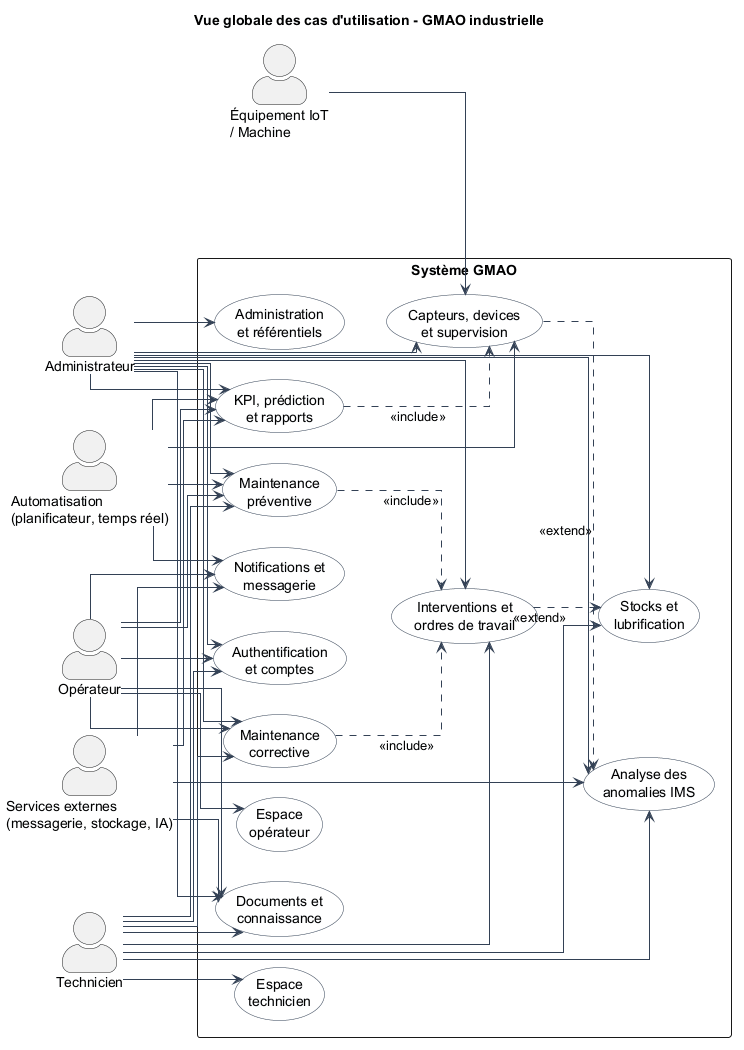
\includegraphics[width=0.98\linewidth,height=0.84\textheight,keepaspectratio]{figures/global-use-case-overview.png}
    \caption{Diagramme global des cas d’utilisation de la plateforme GMAO}
    \label{fig:global-use-case}
\end{figure}
\end{landscape}


Le diagramme global fournit une vue d’ensemble. Afin de présenter toutes les fonctionnalités sans réduire excessivement les libellés, les figures suivantes détaillent les cas d’utilisation par acteur. Les fonctions communes de la figure~\ref{fig:uc-acces-commun} sont héritées par l’administrateur, l’opérateur et le technicien.

\clearpage
\begin{figure}[H]
    \centering
    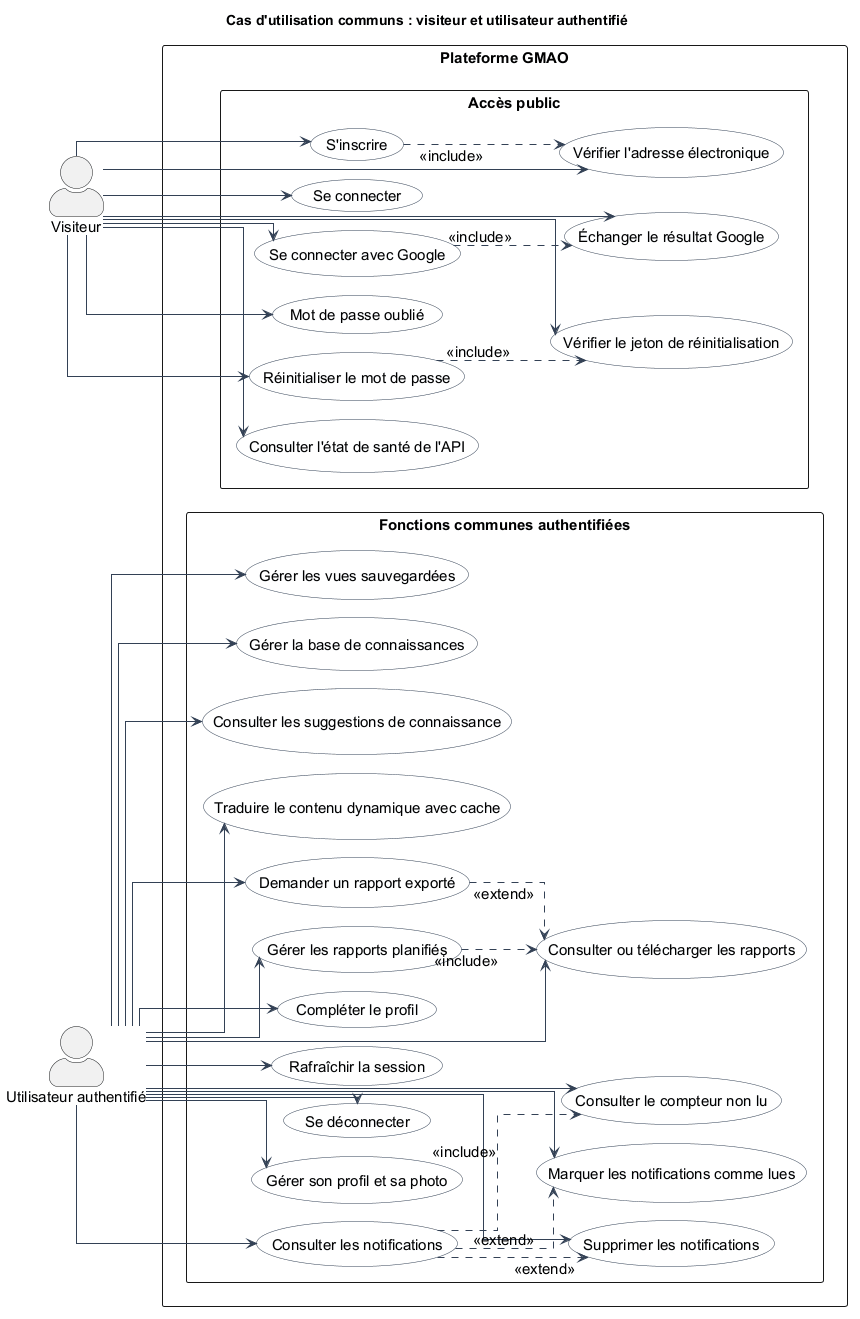
\includegraphics[width=0.94\textwidth,height=0.78\textheight,keepaspectratio]{figures/use-cases/acces-commun.png}
    \caption{Cas d’utilisation du visiteur et fonctions communes aux utilisateurs authentifiés}
    \label{fig:uc-acces-commun}
\end{figure}

\clearpage
\begin{figure}[H]
    \centering
    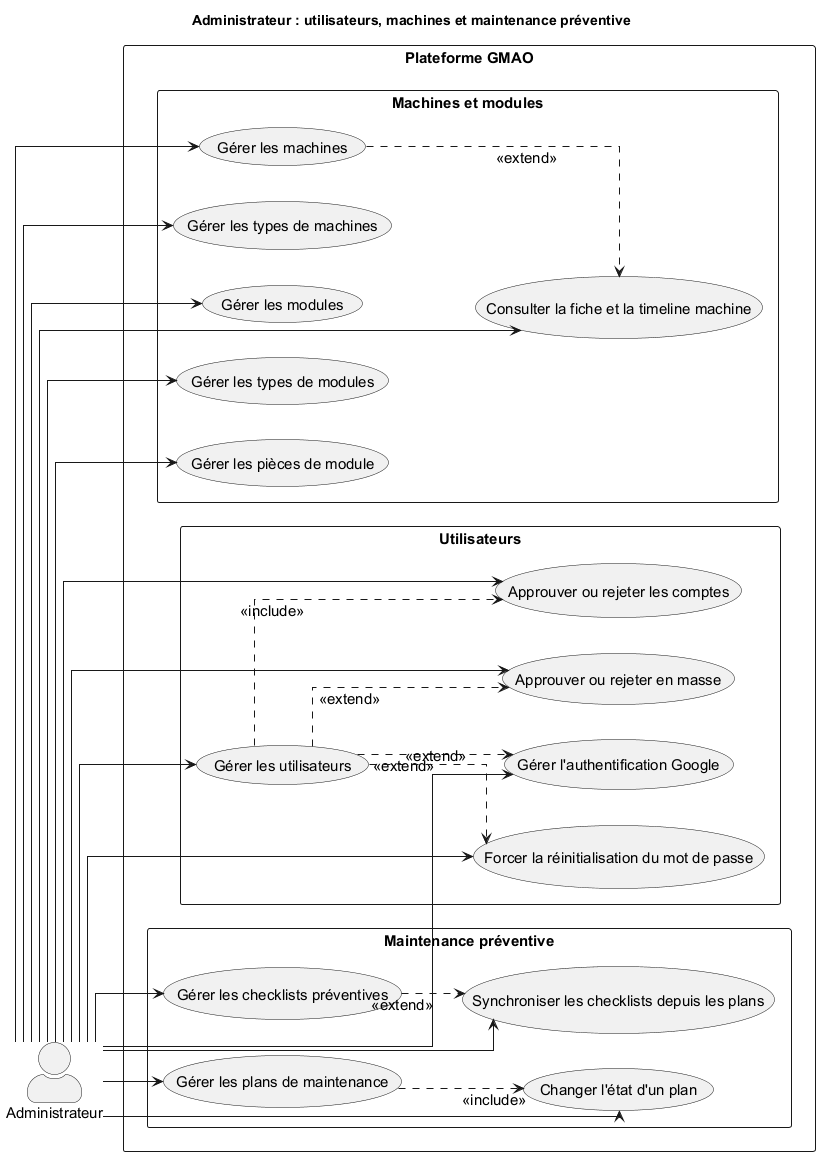
\includegraphics[width=0.94\textwidth,height=0.78\textheight,keepaspectratio]{figures/use-cases/administrateur-referentiels.png}
    \caption{Cas d’utilisation de l’administrateur -- utilisateurs, machines et maintenance préventive}
    \label{fig:uc-administrateur-referentiels}
\end{figure}

\clearpage
\begin{figure}[H]
    \centering
    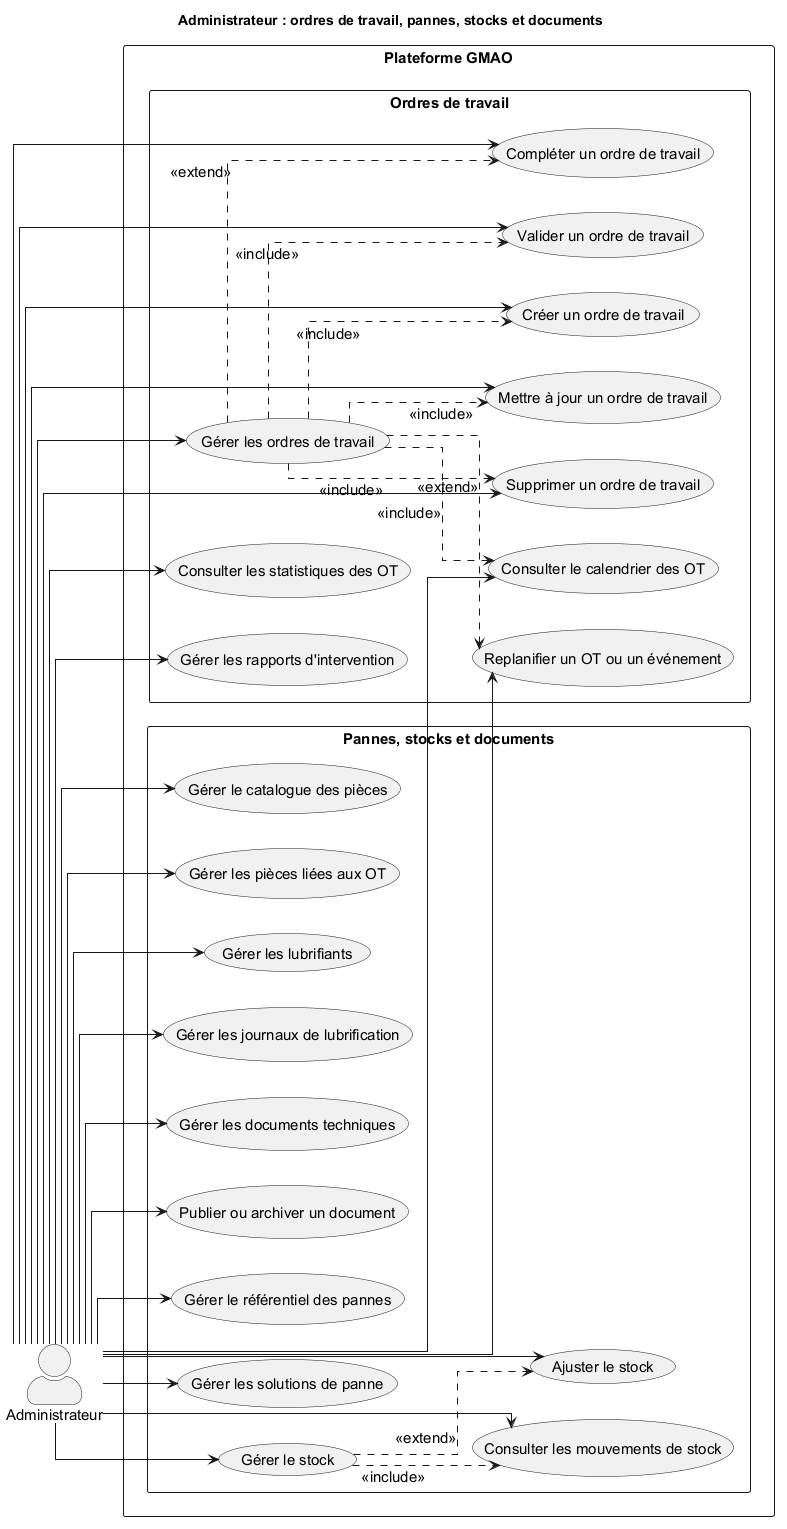
\includegraphics[width=0.94\textwidth,height=0.78\textheight,keepaspectratio]{figures/use-cases/administrateur-operations.png}
    \caption{Cas d’utilisation de l’administrateur -- ordres de travail, pannes, stocks et documents}
    \label{fig:uc-administrateur-operations}
\end{figure}

\clearpage
\begin{figure}[H]
    \centering
    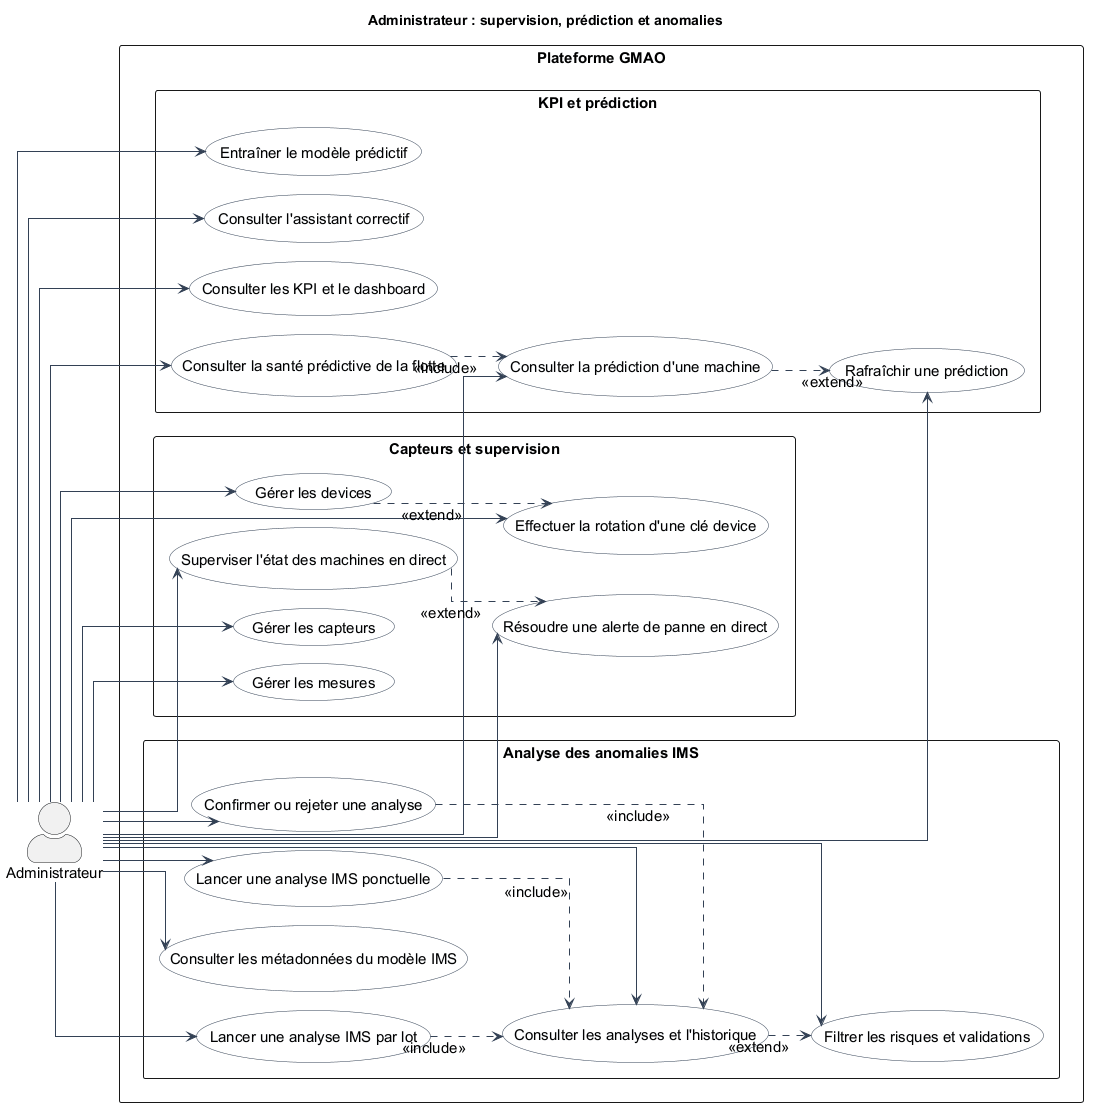
\includegraphics[width=0.94\textwidth,height=0.78\textheight,keepaspectratio]{figures/use-cases/administrateur-2.png}
    \caption{Cas d’utilisation de l’administrateur -- supervision, prédiction et anomalies}
    \label{fig:uc-administrateur-2}
\end{figure}

\clearpage
\begin{figure}[H]
    \centering
    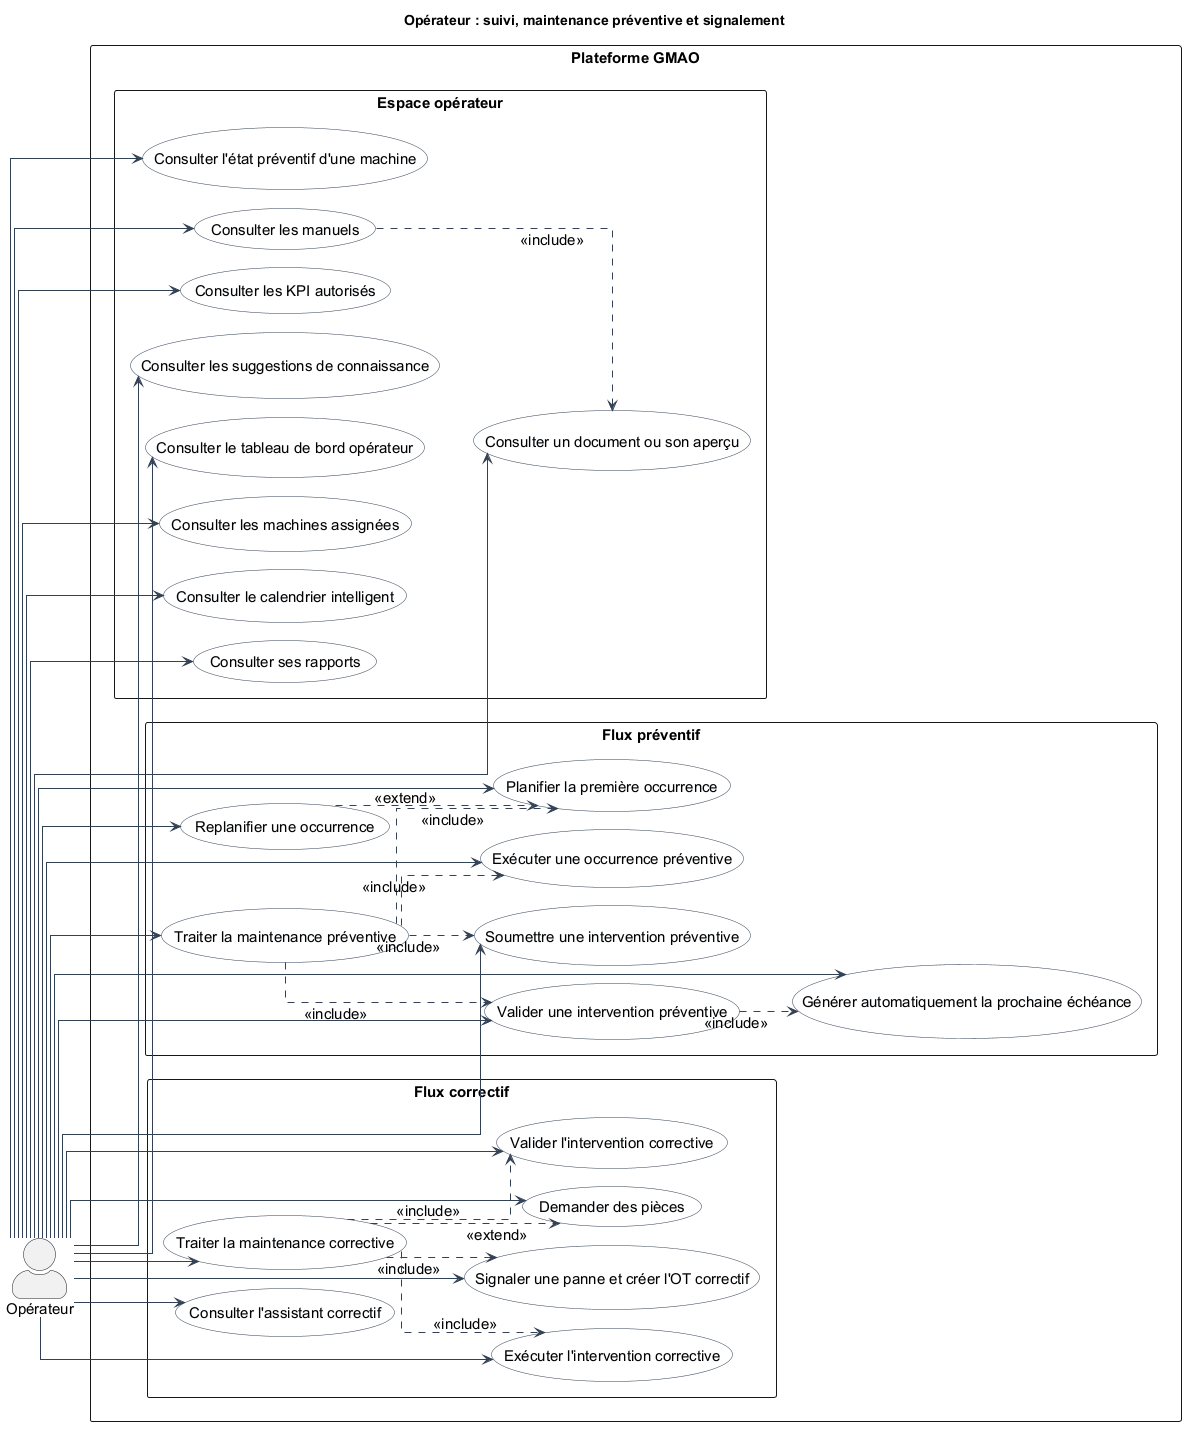
\includegraphics[width=0.94\textwidth,height=0.78\textheight,keepaspectratio]{figures/use-cases/operateur.png}
    \caption{Cas d’utilisation détaillés de l’opérateur}
    \label{fig:uc-operateur}
\end{figure}

\clearpage
\begin{figure}[H]
    \centering
    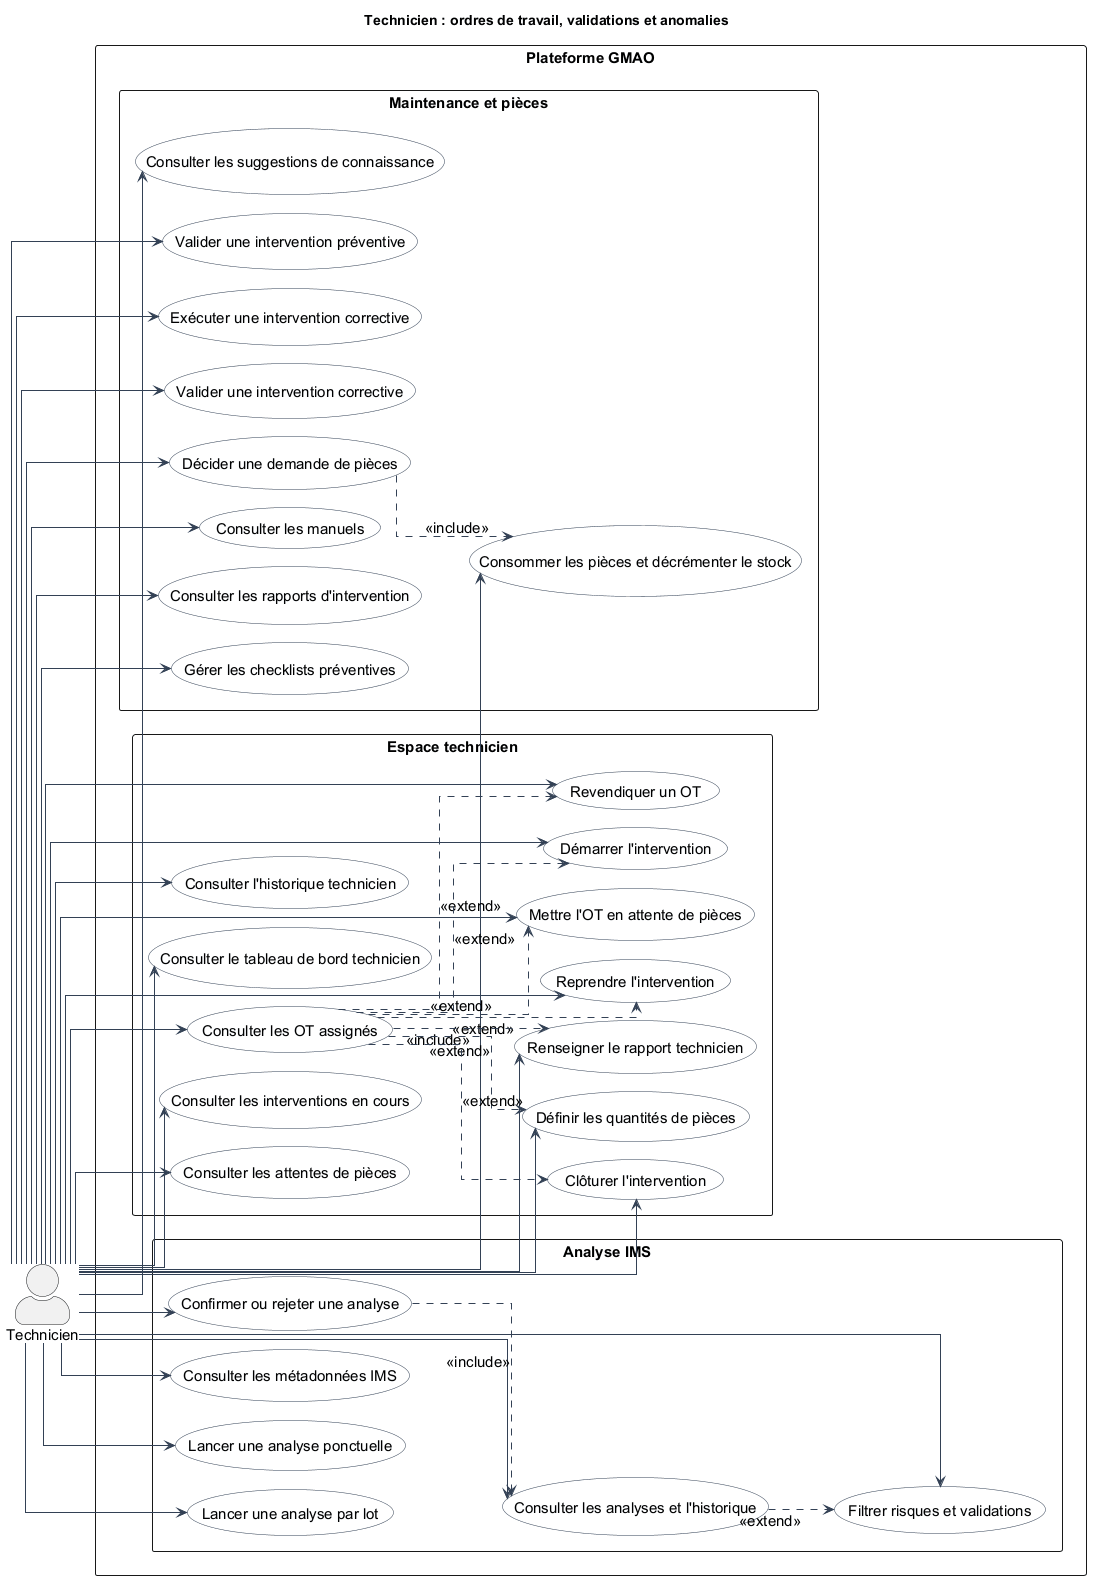
\includegraphics[width=0.94\textwidth,height=0.78\textheight,keepaspectratio]{figures/use-cases/technicien.png}
    \caption{Cas d’utilisation détaillés du technicien}
    \label{fig:uc-technicien}
\end{figure}

\clearpage
\begin{figure}[H]
    \centering
    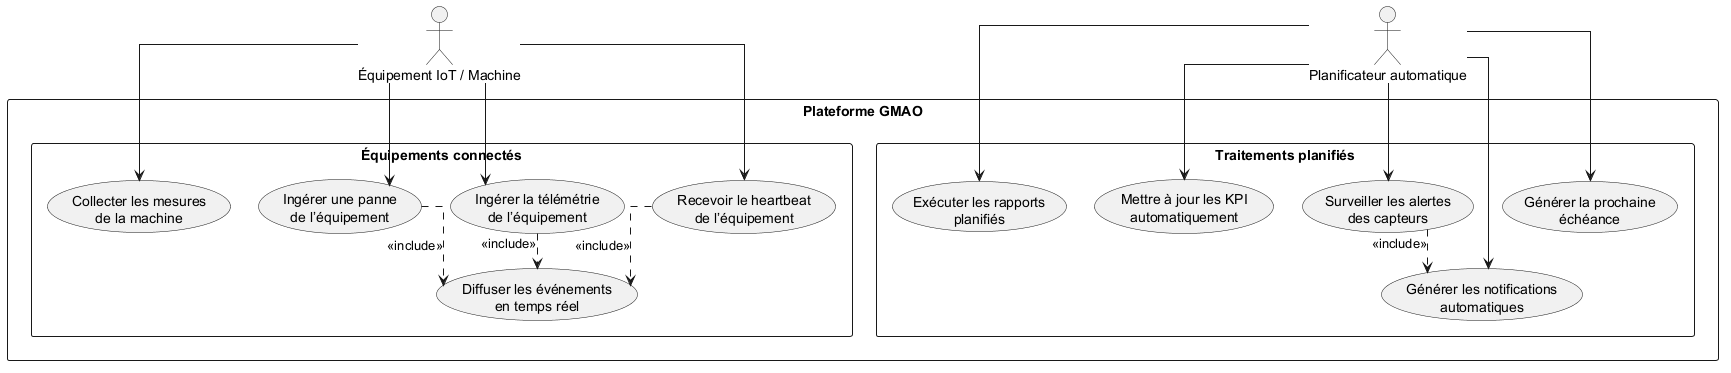
\includegraphics[width=0.94\textwidth,height=0.78\textheight,keepaspectratio]{figures/use-cases/equipements-automatisation.png}
    \caption{Interactions avec les équipements connectés et les traitements automatiques}
    \label{fig:uc-equipements-automatisation}
\end{figure}

\clearpage
\begin{figure}[H]
    \centering
    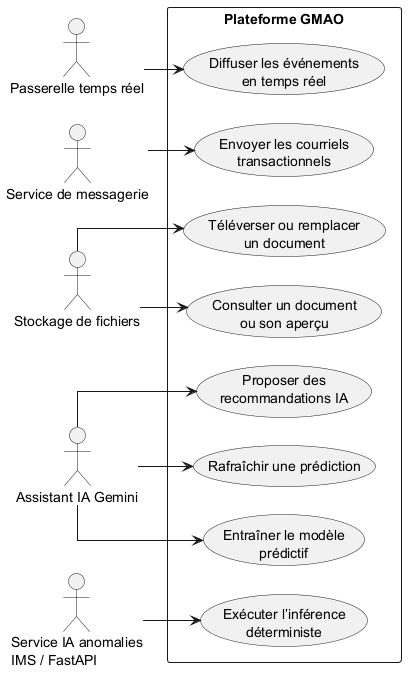
\includegraphics[width=0.94\textwidth,height=0.78\textheight,keepaspectratio]{figures/use-cases/services-externes.png}
    \caption{Interactions avec les services externes de la plateforme}
    \label{fig:uc-services-externes}
\end{figure}


\subsection{Pilotage du projet avec Scrum}

Cette section présente l’application concrète de Scrum au projet. La définition générale de la méthode ayant déjà été exposée dans le chapitre précédent, seuls les rôles, le Product Backlog et la planification des Sprints sont détaillés ici.

\subsubsection{Identification des rôles Scrum}

Dans le contexte de ce projet individuel, les responsabilités de Scrum ont été adaptées aux conditions du stage.

\begin{table}[H]
\centering
\caption{Répartition des responsabilités Scrum}
\label{tab:roles-scrum}
\small
\begin{tabularx}{\textwidth}{|p{3.2cm}|X|}
\hline
\textbf{Responsabilité} & \textbf{Application dans le projet} \\
\hline

Représentation du Product Owner &
L’encadrant professionnel contribue à l’expression des besoins métier, à la définition des priorités et à la validation des résultats. \\
\hline

Scrum Master &
L’étudiante organise le travail, suit l’avancement, identifie les difficultés et adapte la planification lorsque cela est nécessaire. \\
\hline

Développement &
L’étudiante assure l’analyse, la conception, le développement, les tests, la documentation et la préparation du déploiement. \\
\hline
\end{tabularx}
\end{table}

Cette adaptation permet de conserver les principes de transparence, d’inspection et d’adaptation tout en tenant compte du caractère individuel du projet.

\subsubsection{Product Backlog}

Le Product Backlog regroupe et ordonne les fonctionnalités à réaliser. Les besoins sont formulés sous la forme de \textit{User Stories} et répartis selon leur priorité et leurs dépendances fonctionnelles.

Le tableau~\ref{tab:product-backlog} présente une version synthétique du Product Backlog. Les tâches techniques détaillées sont précisées dans les Sprint Backlogs des chapitres correspondants.

\begin{longtable}{|p{0.9cm}|p{9.4cm}|p{1.5cm}|p{1.2cm}|}
\caption{Product Backlog synthétique de la plateforme}
\label{tab:product-backlog}\\
\hline
\textbf{ID} & \textbf{User Story} & \textbf{Priorité} & \textbf{Sprint} \\
\hline
\endfirsthead
\hline
\textbf{ID} & \textbf{User Story} & \textbf{Priorité} & \textbf{Sprint} \\
\hline
\endhead
US01 & En tant qu’utilisateur, je souhaite m’authentifier et gérer mon profil afin d’accéder à la plateforme de manière sécurisée. & Haute & 1 \\
\hline
US02 & En tant qu’administrateur, je souhaite approuver les comptes et gérer les rôles afin de contrôler les accès. & Haute & 1 \\
\hline
US03 & En tant qu’administrateur, je souhaite gérer les machines, leurs types et leurs modules afin de structurer le parc industriel. & Haute & 2 \\
\hline
US04 & En tant qu’utilisateur autorisé, je souhaite consulter les documents techniques et l’historique des machines afin de préparer les interventions. & Moyenne & 2 \\
\hline
US05 & En tant qu’administrateur, je souhaite gérer les plans et les tâches préventives afin de planifier les opérations de maintenance. & Haute & 3 \\
\hline
US06 & En tant qu’opérateur, je souhaite exécuter et soumettre les listes de contrôle afin d’assurer le suivi des opérations préventives. & Haute & 3 \\
\hline
US07 & En tant qu’opérateur, je souhaite signaler une panne afin de déclencher le processus de maintenance corrective. & Haute & 4 \\
\hline
US08 & En tant que technicien, je souhaite prendre en charge et traiter un ordre de travail afin d’assurer le suivi de l’intervention. & Haute & 4 \\
\hline
US09 & En tant que technicien, je souhaite déclarer les pièces utilisées afin d’assurer la traçabilité de leur consommation. & Haute & 4 \\
\hline
US10 & En tant qu’administrateur, je souhaite gérer les pièces et les mouvements de stock afin de suivre leur disponibilité. & Haute & 5 \\
\hline
US11 & En tant qu’utilisateur, je souhaite consulter les notifications, les rapports et les indicateurs correspondant à mon rôle. & Moyenne & 5 \\
\hline
US12 & En tant qu’administrateur, je souhaite superviser les données transmises par les équipements connectés afin de suivre leur état. & Moyenne & 6 \\
\hline
US13 & En tant qu’administrateur ou technicien, je souhaite analyser et valider les anomalies détectées afin de soutenir le diagnostic. & Moyenne & 6 \\
\hline
US14 & En tant qu’utilisateur, je souhaite utiliser, lorsqu’il est activé, un assistant intelligent afin d’obtenir une aide contextuelle. & Faible & 6 \\
\hline
US15 & En tant que responsable du projet, je souhaite automatiser les contrôles de qualité, les tests et le déploiement afin de fiabiliser les livraisons. & Haute & 7 \\
\hline
US16 & En tant que responsable du projet, je souhaite superviser les services déployés afin de détecter et de diagnostiquer les incidents. & Moyenne & 7 \\
\hline
\end{longtable}

\subsubsection{Planification des Sprints}

Les éléments du Product Backlog ont été regroupés selon leurs dépendances et leur cohérence fonctionnelle. Le projet comprend un Sprint 0 d’analyse, suivi de sept Sprints de réalisation.

\begin{table}[H]
\centering
\caption{Planification générale des Sprints}
\label{tab:planification-sprints}
\small
\begin{tabularx}{\textwidth}{|p{1.7cm}|p{4.7cm}|X|}
\hline
\textbf{Sprint} & \textbf{Thème} & \textbf{Objectif principal} \\
\hline
Sprint 0 & Analyse et spécification & Identifier les acteurs et les besoins, constituer le Product Backlog et définir l’architecture générale. \\
\hline
Sprint 1 & Authentification et accès & Sécuriser l’accès et gérer les utilisateurs, les profils, les rôles et les autorisations. \\
\hline
Sprint 2 & Machines et équipements & Structurer les machines, les modules, les historiques et les documents techniques. \\
\hline
Sprint 3 & Maintenance préventive & Gérer les plans, les tâches, les occurrences et le cycle de validation préventif. \\
\hline
Sprint 4 & Maintenance corrective & Traiter les pannes, les interventions, les ordres de travail et les pièces consommées. \\
\hline
Sprint 5 & Stocks et pilotage & Gérer les stocks, les notifications, les rapports, le calendrier et les indicateurs. \\
\hline
Sprint 6 & Surveillance et prédiction & Superviser les équipements connectés et intégrer l’analyse des anomalies. \\
\hline
Sprint 7 & DevSecOps et déploiement & Automatiser les contrôles, déployer les composants et superviser leur fonctionnement. \\
\hline
\end{tabularx}
\end{table}

\subsection{Architecture générale de la solution}

L’architecture de la plateforme organise les composants selon leurs responsabilités et leurs interactions. Elle sépare l’interface utilisateur, les services métier, la persistance des données, les services d’intelligence artificielle et les outils d’exploitation.

Cette organisation modulaire facilite les tests, la maintenance, le déploiement et l’évolution de la solution. L’architecture est présentée selon deux vues complémentaires : une vue logique décrivant les couches applicatives et une vue physique représentant les composants déployés et leurs échanges.

\subsubsection{Architecture logique}

L’architecture logique de la plateforme est organisée autour des couches suivantes :

\begin{description}
    \item[Couche de présentation :] elle correspond à l’application Next.js. Elle affiche les interfaces adaptées aux rôles, assure la navigation et communique avec les services du backend.
    \item[Couche applicative et métier :] elle est mise en œuvre avec NestJS. Elle contient les modules responsables de l’authentification, des utilisateurs, des équipements, de la maintenance, des ordres de travail, des stocks, des documents, des notifications et des rapports.
    \item[Couche de communication :] elle regroupe l’API REST, les WebSockets et le protocole MQTT. L’API traite les opérations applicatives, les WebSockets diffusent les événements en temps réel et MQTT permet l’ingestion des données des équipements connectés.
    \item[Couche d’accès aux données :] elle utilise Mongoose pour assurer la communication entre les modules métier et MongoDB.
    \item[Couche de persistance :] elle comprend MongoDB pour les données métier et Supabase Storage pour le stockage des documents.
    \item[Couche d’intelligence :] elle comprend le service FastAPI chargé de l’analyse des anomalies IMS. Elle peut également communiquer avec Gemini lorsque l’assistant intelligent est activé.
    \item[Couche d’exploitation :] elle regroupe la planification automatique, la production des métriques, la journalisation et les mécanismes de supervision.
\end{description}

La figure~\ref{fig:architecture-logique} présente l’organisation logique de ces composants.

\begin{figure}[H]
    \centering
    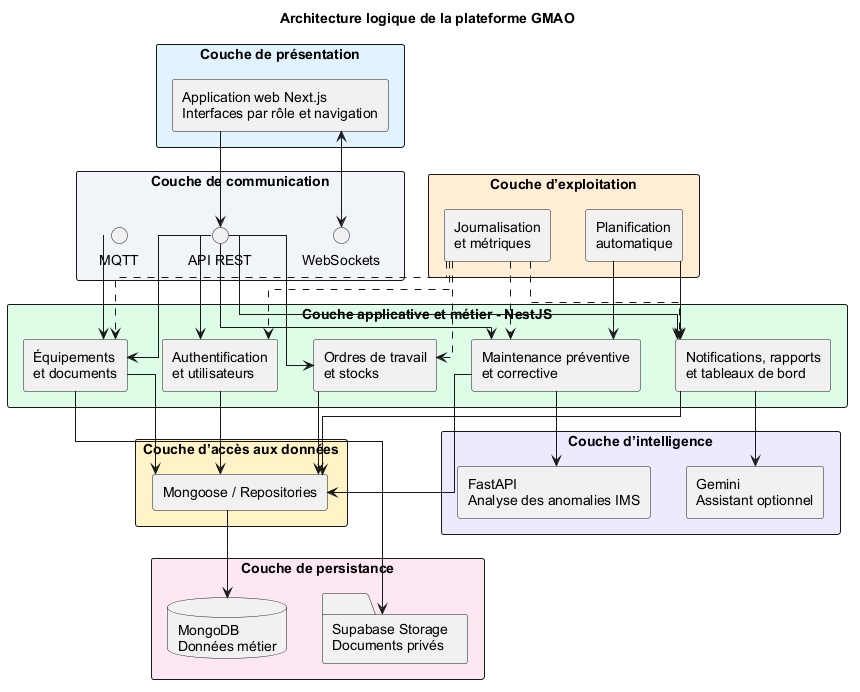
\includegraphics[width=\textwidth,height=0.72\textheight,keepaspectratio]{figures/architecture-logique.png}
    \caption{Architecture logique de la plateforme GMAO}
    \label{fig:architecture-logique}
\end{figure}

\subsubsection{Architecture physique}

L’architecture physique représente l’environnement de déploiement et les échanges entre les différents composants de la plateforme.

Les utilisateurs accèdent à l’interface Next.js déployée sur Vercel depuis un navigateur web. Cette interface communique en HTTPS avec l’API NestJS déployée sur Render. Le backend applique les règles métier, contrôle les autorisations et orchestre les échanges avec les services de données et les intégrations externes.

Les données métier sont conservées dans MongoDB Atlas, tandis que les documents téléversés sont stockés dans un espace privé Supabase Storage. L’accès aux fichiers est contrôlé par le backend afin d’éviter l’exposition des informations d’authentification du service de stockage.

Le service FastAPI chargé de l’analyse des anomalies IMS est également déployé sur Render. Il est appelé uniquement par le backend à travers une communication authentifiée par un jeton de service. Le navigateur ne communique donc pas directement avec le modèle d’analyse.

La plateforme peut également communiquer avec un courtier MQTT pour recevoir les données des équipements connectés, avec un service de messagerie pour l’envoi des courriels et avec Gemini lorsque l’assistant optionnel est activé.

Enfin, Prometheus collecte les métriques exposées par le backend, tandis que Grafana permet leur visualisation. Les détails relatifs au déploiement, à la chaîne CI/CD, à la sécurité des secrets et à la supervision seront présentés dans le Sprint 7.

\begin{figure}[H]
    \centering
    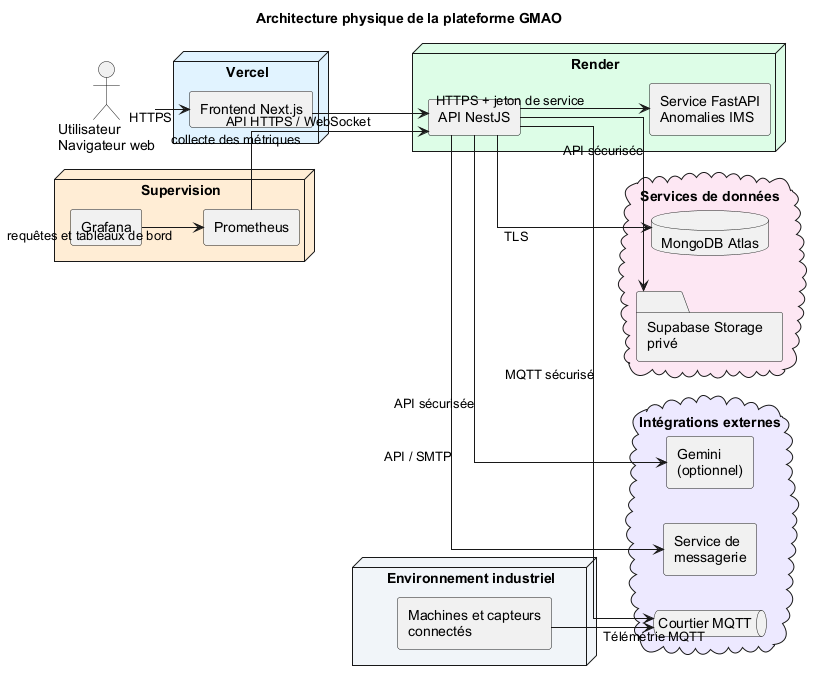
\includegraphics[width=\textwidth,height=0.72\textheight,keepaspectratio]{figures/architecture-physique.png}
    \caption{Architecture physique de la plateforme GMAO}
    \label{fig:architecture-physique}
\end{figure}

\iffalse

Le \textit{Product Backlog} représente la liste ordonnée de l'ensemble des fonctionnalités à développer afin de répondre aux besoins identifiés durant la phase d'analyse. Dans le cadre de la méthode Scrum, il constitue un artefact central regroupant les exigences fonctionnelles du projet sous forme de \textit{User Stories}. Chaque fonctionnalité est priorisée selon sa valeur métier et son importance pour les utilisateurs.

Le Product Backlog a été élaboré en collaboration avec les responsables de l'entreprise afin de planifier progressivement le développement de la plateforme. Les fonctionnalités ont ensuite été réparties sur plusieurs sprints en fonction de leur priorité et de leur dépendance.

Le tableau \ref{tab:product-backlog} présente une synthèse des principales fonctionnalités retenues pour le développement de la plateforme.

\begin{table}[H]
\centering
\renewcommand{\arraystretch}{1.3}
\small
\begin{tabular}{|c|p{6cm}|c|c|}
\hline
\textbf{ID} &
\textbf{User Story} &
\textbf{Priorité} &
\textbf{Sprint}
\\
\hline

US01 &
En tant qu'utilisateur, je souhaite m'authentifier afin d'accéder à la plateforme de manière sécurisée. &
Haute &
1
\\
\hline

US02 &
En tant qu'administrateur, je souhaite gérer les utilisateurs afin d'administrer les accès au système. &
Haute &
2
\\
\hline

US03 &
En tant qu'utilisateur, je souhaite gérer mon profil afin de mettre à jour mes informations personnelles. &
Moyenne &
2
\\
\hline

US04 &
En tant qu'administrateur, je souhaite gérer les machines afin de centraliser les équipements industriels. &
Haute &
3
\\
\hline

US05 &
En tant qu'administrateur, je souhaite gérer les modules des machines afin de structurer les équipements. &
Haute &
3
\\
\hline

US06 &
En tant qu'administrateur, je souhaite gérer les documents techniques afin de faciliter les interventions. &
Moyenne &
3
\\
\hline

US07 &
En tant qu'opérateur, je souhaite effectuer les opérations de maintenance préventive afin de réduire les risques de panne. &
Haute &
4
\\
\hline

US08 &
En tant qu'opérateur, je souhaite déclarer une panne afin de déclencher une intervention corrective. &
Haute &
4
\\
\hline

US09 &
En tant que technicien, je souhaite valider les rapports d'intervention afin d'assurer le suivi des opérations. &
Haute &
4
\\
\hline

US10 &
En tant qu'utilisateur, je souhaite consulter le tableau de bord afin de suivre les indicateurs de maintenance. &
Moyenne &
5
\\
\hline

US11 &
En tant qu'utilisateur, je souhaite consulter le calendrier de maintenance afin de connaître les interventions programmées. &
Moyenne &
5
\\
\hline

US12 &
En tant qu'utilisateur, je souhaite utiliser un assistant intelligent afin d'obtenir une aide contextuelle lors des opérations de maintenance. &
Faible &
6
\\
\hline

\end{tabular}

\caption{Product Backlog de la plateforme}
\label{tab:product-backlog}

\end{table} 

Le Product Backlog présenté ci-dessus constitue une vision synthétique des principales fonctionnalités de la plateforme. Chaque fonctionnalité a été transformée en une ou plusieurs \textit{User Stories}, puis planifiée dans un sprint en fonction de sa priorité métier et de sa dépendance vis-à-vis des autres fonctionnalités.

Cette organisation a permis de développer progressivement l'application tout en validant chaque incrément avant le démarrage du sprint suivant. Elle a également facilité l'intégration des retours formulés par les responsables de l'entreprise au cours du développement.

\subsubsection{Planification des Sprints}

Les éléments du Product Backlog ont été répartis en Sprints selon leur priorité, leurs dépendances et leur cohérence fonctionnelle. Cette planification progressive permet de produire un incrément vérifiable à la fin de chaque Sprint, d’intégrer les retours de l’encadrement et d’ajuster les travaux suivants lorsque cela est nécessaire.

\subsection{Architecture générale de la solution}

L'architecture générale d'un système définit l'organisation des différents composants logiciels ainsi que leurs interactions. Elle constitue un élément essentiel de la conception puisqu'elle permet d'assurer une séparation claire des responsabilités, une meilleure évolutivité ainsi qu'une maintenance facilitée de l'application.

Dans le cadre de ce projet, une architecture client--serveur a été retenue. Cette architecture repose sur une séparation entre l'interface utilisateur, la logique métier et la couche de persistance des données. Cette organisation favorise la modularité de l'application, améliore sa maintenabilité et facilite son déploiement sur des infrastructures cloud.

L'architecture générale de la plateforme est présentée selon deux points de vue complémentaires : l'architecture physique, qui décrit le déploiement des différents composants, et l'architecture logique, qui illustre leur organisation fonctionnelle.

\subsubsection{Architecture logique}

L'architecture logique décrit l'organisation interne des différents composants logiciels de la plateforme ainsi que leurs responsabilités respectives. Elle permet de représenter les différentes couches applicatives indépendamment de leur déploiement physique.

La solution développée repose sur une architecture multicouche composée principalement d'une couche de présentation, d'une couche métier, d'une couche d'accès aux données ainsi que d'une couche de persistance.

La couche de présentation correspond à l'application web développée avec Next.js. Elle assure les interactions avec les utilisateurs et permet l'affichage dynamique des informations.

La couche métier est implémentée au sein du backend NestJS. Elle regroupe l'ensemble des services responsables de la gestion des utilisateurs, des équipements, des interventions de maintenance, des documents techniques, des tableaux de bord ainsi que des autres fonctionnalités de la plateforme.

La couche d'accès aux données assure la communication entre les services métier et la base de données MongoDB à travers les différents modèles de données.

Enfin, la couche de persistance garantit le stockage durable des informations manipulées par l'application.


\begin{figure}[H]
\centering

\includegraphics[width=.90\textwidth]{figures/logical-architecture.jpg}
\caption{Architecture logique de la plateforme}
\label{fig:logical-architecture}
\end{figure}


Cette architecture multicouche permet de limiter le couplage entre les différents composants de l'application tout en améliorant leur réutilisabilité. Chaque couche possède une responsabilité clairement définie, ce qui facilite les opérations de maintenance, les évolutions futures ainsi que l'intégration de nouvelles fonctionnalités.

Par ailleurs, cette organisation favorise le développement collaboratif en permettant aux différentes parties de l'application d'évoluer indépendamment les unes des autres, tout en garantissant une communication cohérente entre les différents composants du système.

Cette architecture multicouche permet de limiter le couplage entre les différents composants de l'application tout en améliorant leur réutilisabilité. Chaque couche possède une responsabilité clairement définie, ce qui facilite les opérations de maintenance, les évolutions futures ainsi que l'intégration de nouvelles fonctionnalités.

Par ailleurs, cette organisation favorise le développement collaboratif en permettant aux différentes parties de l'application d'évoluer indépendamment les unes des autres, tout en garantissant une communication cohérente entre les différents composants du système.

\subsubsection{Architecture physique}

L'architecture physique décrit l'organisation matérielle et logicielle des différents composants intervenant dans le fonctionnement de la plateforme. Elle met en évidence les échanges entre les utilisateurs, l'interface web, le serveur applicatif ainsi que la base de données.

Dans la solution développée, les utilisateurs accèdent à la plateforme depuis un navigateur web. Les requêtes sont envoyées vers l'application frontend développée avec Next.js. Celle-ci communique avec une API REST réalisée avec NestJS, responsable du traitement des requêtes, de l'application des règles métier, de l'authentification des utilisateurs ainsi que de la gestion des données.

L'ensemble des informations relatives aux utilisateurs, aux équipements, aux interventions de maintenance, aux documents techniques ainsi qu'aux autres ressources est stocké dans une base de données MongoDB Atlas. La plateforme intègre également un service d'authentification sécurisé ainsi qu'un assistant intelligent permettant d'assister les utilisateurs lors de leurs opérations de maintenance.

La figure \ref{fig:physical-architecture} présente l'architecture physique de la plateforme.

\begin{figure}[H]
\centering

\includegraphics[width=\textwidth]{figures/physical-architecture.jpg}
\caption{Architecture physique de la plateforme}
\label{fig:physical-architecture}
\end{figure}

Le frontend constitue le point d'entrée principal de la plateforme. Il assure l'affichage des interfaces utilisateurs ainsi que les échanges avec le serveur via des requêtes HTTP sécurisées.

Le backend centralise la logique métier de l'application. Il traite les demandes provenant des différents utilisateurs, applique les règles de gestion, contrôle les autorisations d'accès et assure la communication avec la base de données.

MongoDB Atlas assure le stockage persistant des données de la plateforme. Cette solution NoSQL permet de gérer efficacement des données hétérogènes tout en offrant une grande flexibilité d'évolution.

Enfin, un module d'assistance intelligente peut être intégré afin d'accompagner les utilisateurs dans leurs activités quotidiennes de maintenance en fournissant des recommandations adaptées au contexte des interventions.

\fi

\subsubsection{Technologies adoptées}

Les technologies ont été sélectionnées selon les besoins fonctionnels, les contraintes de sécurité, la modularité recherchée et les possibilités de déploiement de la plateforme. Le tableau~\ref{tab:technologies} présente les principaux choix techniques.

\begin{table}[H]
\centering
\caption{Principales technologies de la plateforme}
\label{tab:technologies}
\small
\begin{tabularx}{\textwidth}{|p{3.4cm}|p{3.2cm}|X|}
\hline
\textbf{Domaine} & \textbf{Technologie} & \textbf{Utilisation dans le projet} \\
\hline
Langage principal & TypeScript & Développement de l’interface Next.js et de l’API NestJS avec un typage statique. \\
\hline
Interface web & Next.js, React et Tailwind CSS & Construction des interfaces, des tableaux de bord, de la navigation et des composants responsifs. \\
\hline
Services métier & NestJS & Développement de l’API REST, des modules métier, de l’authentification, de la planification et des services applicatifs. \\
\hline
Base de données & MongoDB Atlas et Mongoose & Stockage des données métier et définition des schémas, des validations et des références entre documents. \\
\hline
Temps réel et IoT & Socket.IO et MQTT & Diffusion des événements en temps réel et réception des données provenant des équipements connectés. \\
\hline
Service d’analyse & Python, FastAPI et scikit-learn & Exposition du modèle de détection des anomalies IMS à travers un service indépendant. \\
\hline
Stockage documentaire & Supabase Storage & Conservation sécurisée des documents et des fichiers téléversés. \\
\hline
Visualisation et rapports & Recharts, PDFKit et ExcelJS & Affichage des indicateurs et génération de rapports aux formats PDF et Excel. \\
\hline
Tests et qualité & Jest, Playwright, ESLint et SonarCloud & Tests du backend et du frontend, vérification du code et analyse de la qualité. \\
\hline
Déploiement et supervision & Vercel, Render, Prometheus et Grafana & Déploiement des services, collecte des métriques et visualisation de l’état de la plateforme. \\
\hline
\end{tabularx}
\end{table}

Next.js a été utilisé avec son \textit{App Router} pour structurer les pages et les interfaces de l’application \cite{nextjs_docs}. NestJS fournit une organisation modulaire adaptée à la séparation des domaines métier du backend \cite{nestjs_docs}. MongoDB Atlas assure l’hébergement de la base de données orientée documents \cite{mongodb_atlas_docs}, tandis que FastAPI expose les opérations d’inférence du modèle d’analyse d’anomalies \cite{fastapi_docs}.

Les mécanismes de déploiement, de test, de contrôle de la qualité et de supervision seront détaillés dans le Sprint 7 consacré au DevSecOps.

\iffalse

La réalisation de cette plateforme a nécessité l'utilisation d'un ensemble de technologies modernes permettant de concevoir une application web performante, sécurisée et évolutive. Le choix de ces outils a été effectué en tenant compte des besoins du projet, des performances attendues ainsi que de leur compatibilité avec une architecture web moderne.

L'environnement de développement retenu repose principalement sur une architecture client--serveur. Il combine des langages de programmation, des frameworks, des outils de développement ainsi que des plateformes de déploiement permettant d'assurer l'ensemble du cycle de vie de l'application.

\paragraph{Langages utilisés}

Le développement de la plateforme repose sur plusieurs langages de programmation, chacun étant utilisé selon son domaine d'application.

\begin{itemize}

\item \textbf{TypeScript} : utilisé pour le développement du frontend et du backend. Son typage statique améliore la qualité du code, facilite la détection des erreurs et rend le projet plus maintenable.

\item \textbf{JavaScript} : utilisé par certains outils de configuration ainsi que par plusieurs bibliothèques de l'écosystème Node.js.

\item \textbf{HTML5} : utilisé pour structurer les différentes interfaces de l'application.

\item \textbf{CSS3} : utilisé pour la mise en forme graphique des interfaces utilisateurs.

\item \textbf{SQL (langage de requête)} : utilisé lors de l'analyse comparative des systèmes de gestion de bases de données, bien que la plateforme repose sur MongoDB, une base de données NoSQL.

\end{itemize} 
\begin{table}[H]
\centering
\renewcommand{\arraystretch}{1.3}
\begin{tabular}{|l|p{8cm}|}
\hline
\textbf{Langage} & \textbf{Utilisation} \\
\hline
TypeScript & Développement Frontend et Backend\\
\hline
JavaScript & Configuration et bibliothèques Node.js\\
\hline
HTML5 & Structure des interfaces web\\
\hline
CSS3 & Mise en forme graphique\\
\hline
\end{tabular}
\caption{Langages utilisés}
\label{tab:langages}
\end{table}

\paragraph{Frameworks}

Afin de garantir une architecture logicielle robuste, plusieurs frameworks ont été utilisés au cours du développement de la plateforme.

\fi

\subsubsection{Modèle de données et diagramme de classes}

Le diagramme de classes représente la structure conceptuelle de la plateforme et les principales relations entre les entités métier. Afin de préserver sa lisibilité, la figure~\ref{fig:diagramme-classes} présente une vue synthétique du modèle. Le diagramme technique issu de l’audit d’implémentation est ensuite décliné en six vues fonctionnelles dans les figures~\ref{fig:diagramme-classes-detaille-1} à~\ref{fig:diagramme-classes-detaille-6}.

Les principales entités sont regroupées selon les domaines suivants :

\begin{itemize}
    \item \textbf{identité et accès :} \texttt{User} et les rôles associés ;
    \item \textbf{équipements :} \texttt{MachineType}, \texttt{Machine}, \texttt{ModuleType}, \texttt{Module}, \texttt{Capteur} et \texttt{Mesure} ;
    \item \textbf{maintenance :} \texttt{MaintenancePlan}, \texttt{WorkOrder}, \texttt{InterventionReport} et \texttt{KPI} ;
    \item \textbf{stocks et documents :} \texttt{Catalogue}, \texttt{Stock}, \texttt{PartRequest} et \texttt{DocumentEntity} ;
    \item \textbf{pilotage :} \texttt{Notification} et les services de génération des rapports et de planification ;
    \item \textbf{maintenance prédictive :} \texttt{MachineHealthPrediction}, \texttt{AiAnomalyAnalysis} et \texttt{AiInteraction}.
\end{itemize}

Une machine appartient à un type et peut contenir plusieurs modules. Les modules peuvent être associés à des capteurs, des mesures et des plans de maintenance. Les ordres de travail sont liés aux machines, aux techniciens et, selon leur origine, à un plan préventif. Les rapports d’intervention et les demandes de pièces sont rattachés aux ordres de travail correspondants.

Les analyses d’anomalies sont associées à une machine et, lorsqu’il est identifié, à un capteur. Elles conservent le score de risque, la version du modèle et l’état de validation humaine. Cette organisation permet de retracer les résultats produits et les décisions prises par les administrateurs ou les techniciens.

MongoDB étant une base orientée documents, les relations UML sont implémentées au moyen de références entre documents ou de données imbriquées selon les besoins du domaine.

\begin{landscape}
\begin{figure}[H]
    \centering
    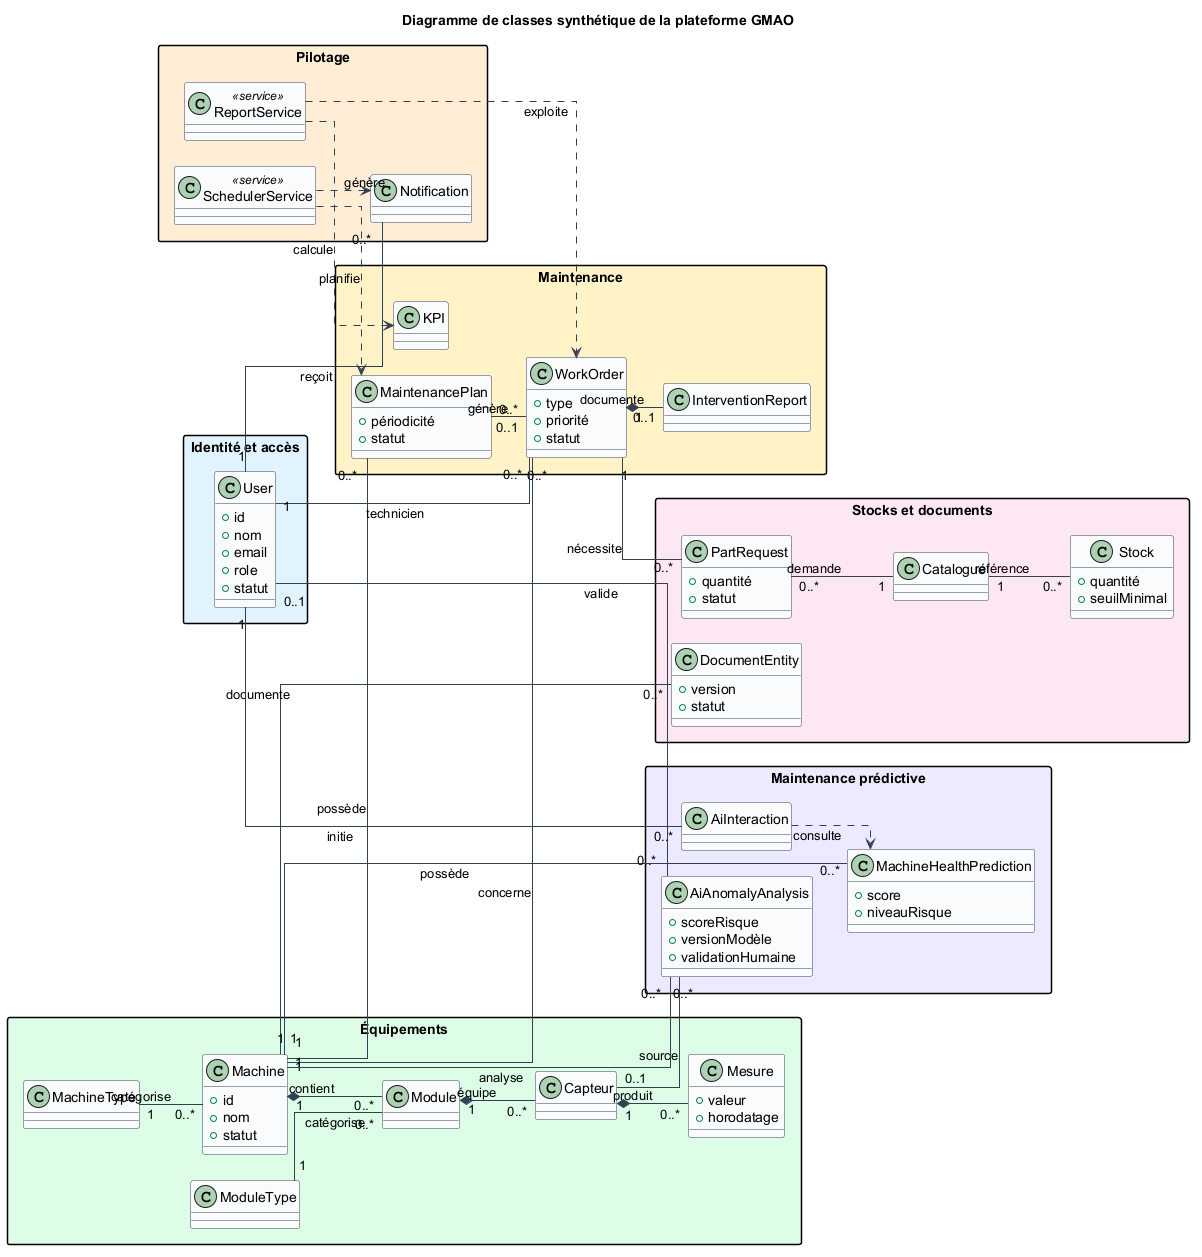
\includegraphics[width=0.96\linewidth,height=0.87\textheight,keepaspectratio]{figures/class-diagram-executive.png}
    \caption{Diagramme de classes synthétique de la plateforme GMAO}
    \label{fig:diagramme-classes}
\end{figure}
\end{landscape}

\begin{landscape}
\begin{figure}[H]
    \centering
    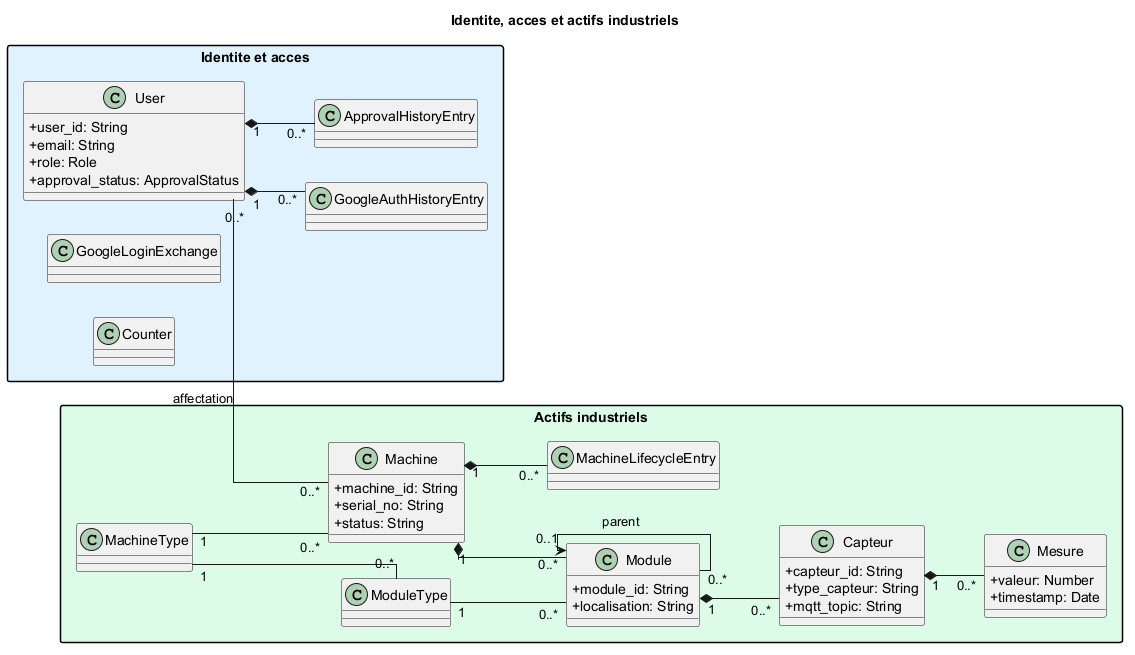
\includegraphics[width=0.97\linewidth,height=0.84\textheight,keepaspectratio]{figures/class-domain-identite-actifs.png}
    \caption{Diagramme de classes -- identité, accès et actifs industriels}
    \label{fig:diagramme-classes-detaille-1}
\end{figure}
\clearpage
\begin{figure}[H]
    \centering
    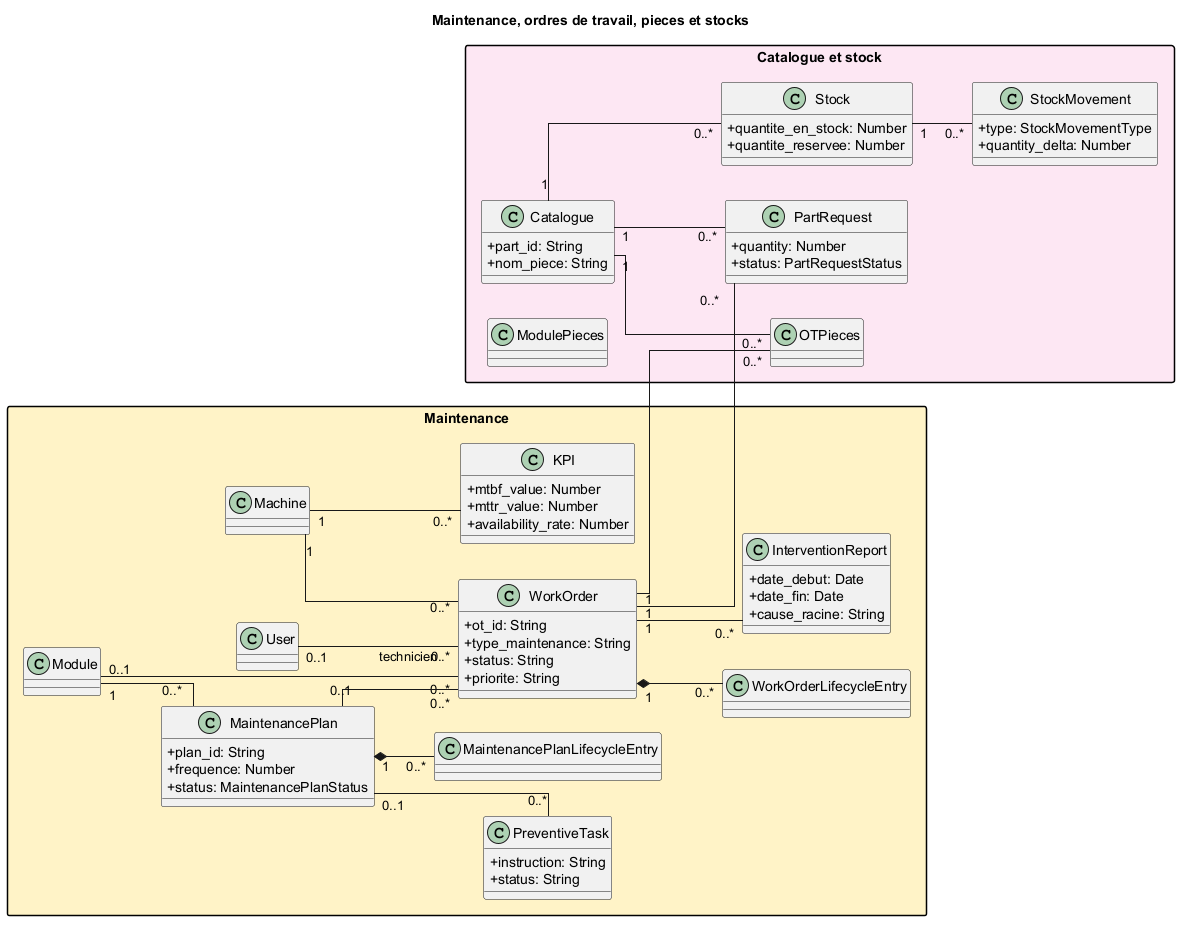
\includegraphics[width=0.97\linewidth,height=0.84\textheight,keepaspectratio]{figures/class-domain-maintenance-stock.png}
    \caption{Diagramme de classes -- maintenance, ordres de travail et stocks}
    \label{fig:diagramme-classes-detaille-2}
\end{figure}
\clearpage
\begin{figure}[H]
    \centering
    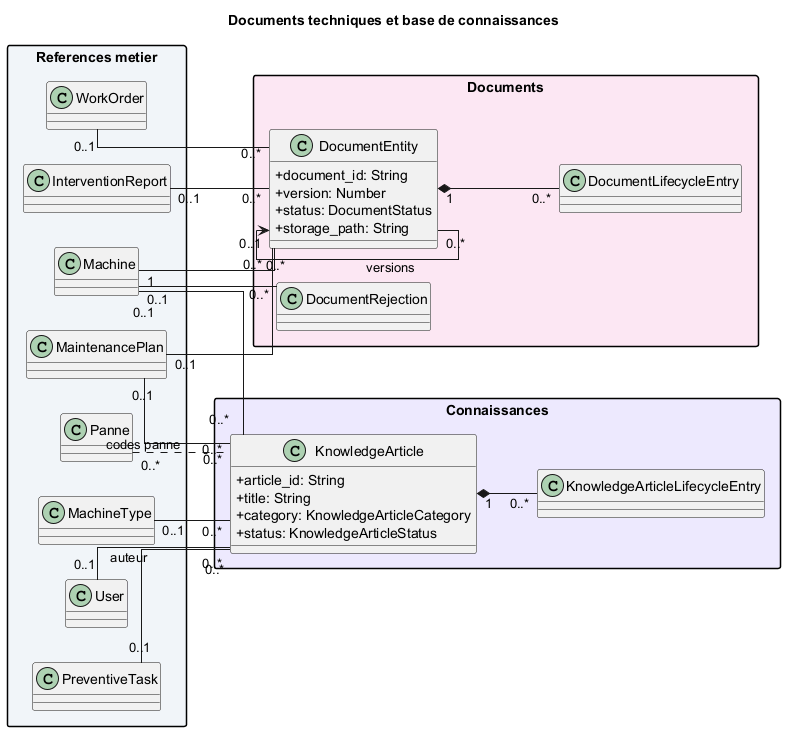
\includegraphics[width=0.97\linewidth,height=0.84\textheight,keepaspectratio]{figures/class-domain-documents.png}
    \caption{Diagramme de classes -- documents et base de connaissances}
    \label{fig:diagramme-classes-detaille-3}
\end{figure}
\clearpage
\begin{figure}[H]
    \centering
    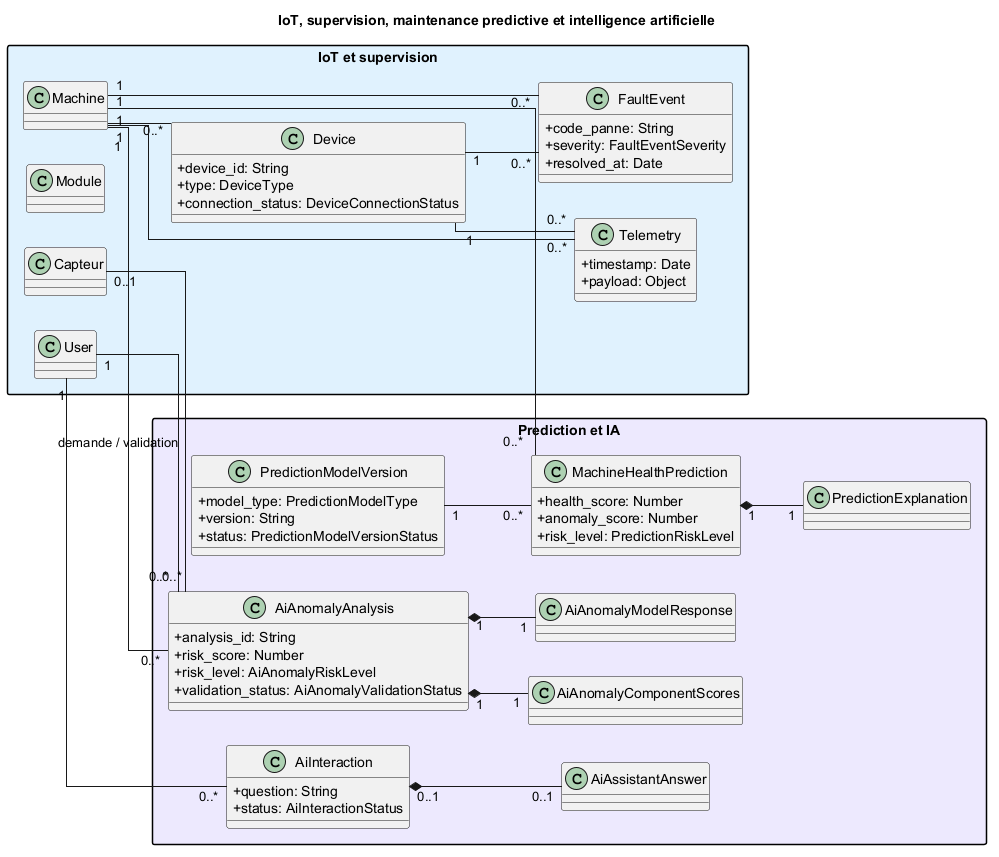
\includegraphics[width=0.97\linewidth,height=0.84\textheight,keepaspectratio]{figures/class-domain-iot-ia.png}
    \caption{Diagramme de classes -- IoT, prédiction et intelligence artificielle}
    \label{fig:diagramme-classes-detaille-4}
\end{figure}
\clearpage
\begin{figure}[H]
    \centering
    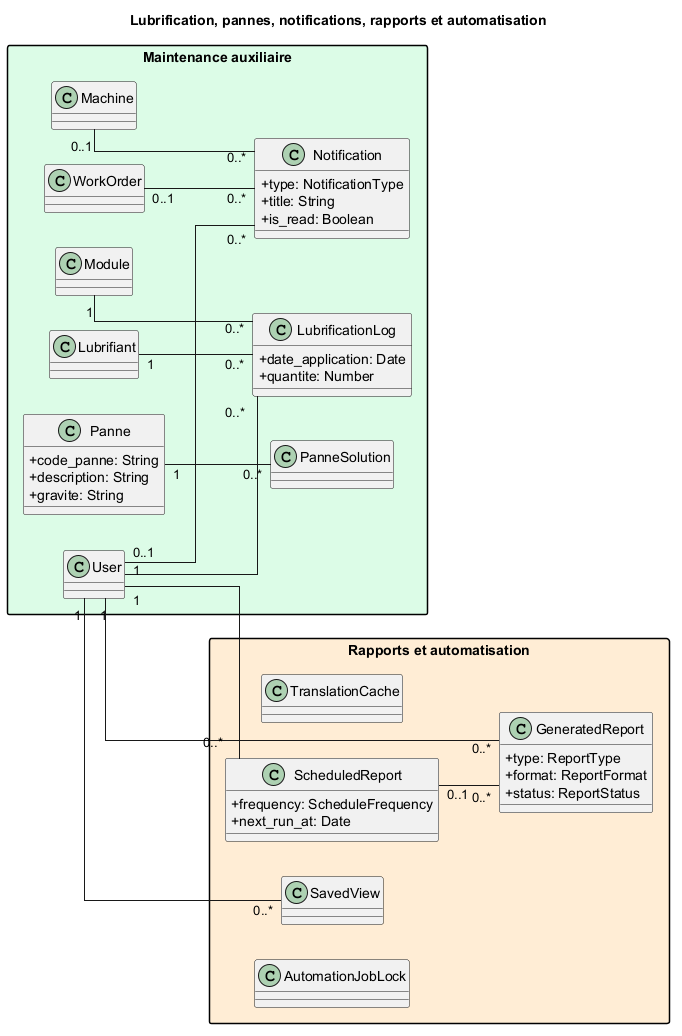
\includegraphics[width=0.97\linewidth,height=0.84\textheight,keepaspectratio]{figures/class-domain-pilotage.png}
    \caption{Diagramme de classes -- maintenance auxiliaire, rapports et automatisation}
    \label{fig:diagramme-classes-detaille-5}
\end{figure}
\clearpage
\begin{figure}[H]
    \centering
    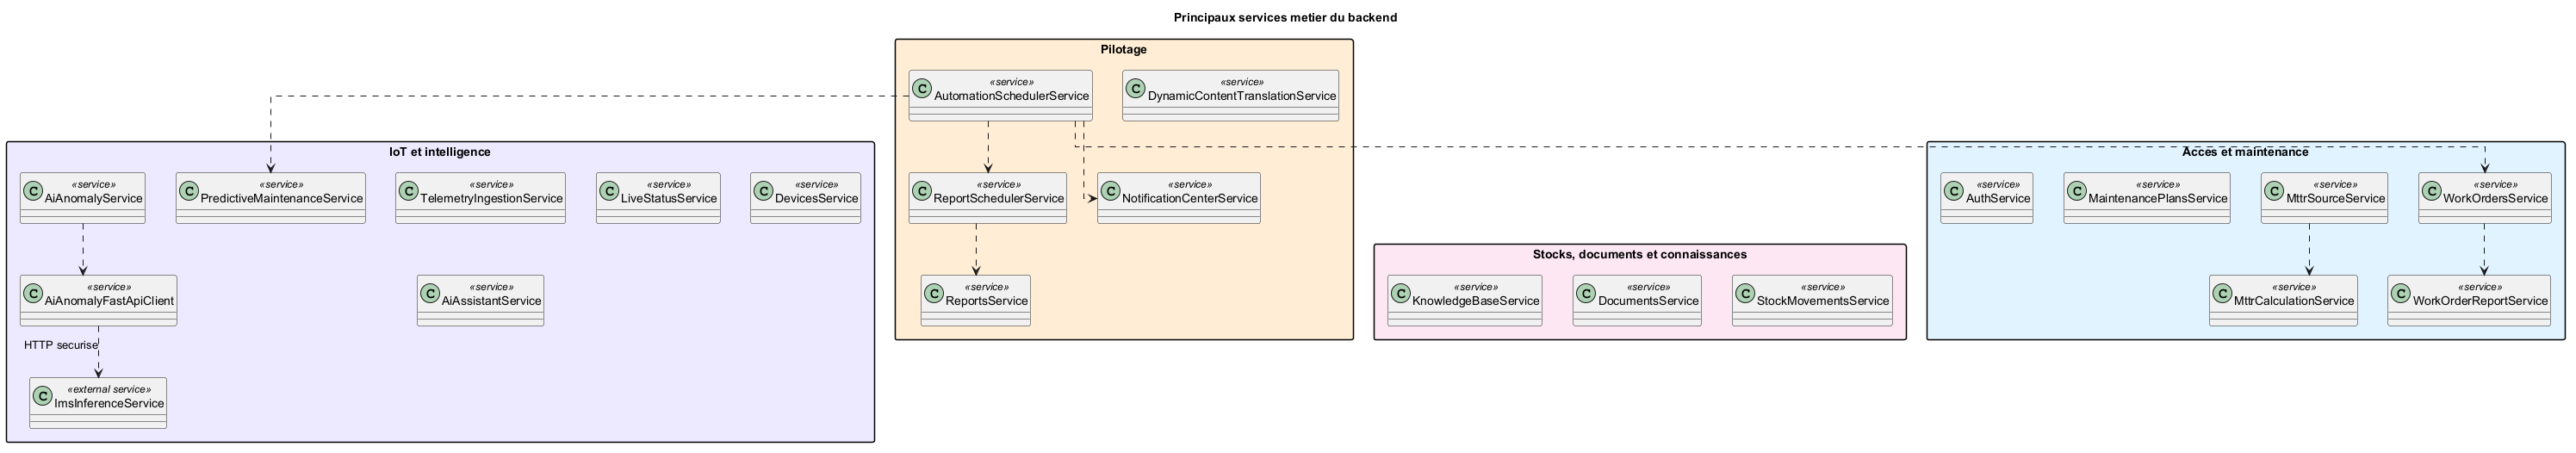
\includegraphics[width=0.97\linewidth,height=0.84\textheight,keepaspectratio]{figures/class-domain-services.png}
    \caption{Diagramme de classes -- principaux services métier du backend}
    \label{fig:diagramme-classes-detaille-6}
\end{figure}
\end{landscape}

\iffalse

Le diagramme de classes constitue l'un des principaux diagrammes de la modélisation UML. Il permet de représenter la structure statique du système en identifiant les différentes classes, leurs attributs, leurs opérations ainsi que les relations existantes entre elles. Cette modélisation facilite la compréhension de l'organisation des données et constitue une référence importante lors des phases de conception et de développement de l'application.

Dans le cadre de ce projet, le diagramme de classes a été élaboré à partir des besoins fonctionnels identifiés précédemment. Il représente les principales entités manipulées par la plateforme de gestion de la maintenance industrielle ainsi que les liens qui les unissent.

La structure retenue repose sur une architecture modulaire permettant d'assurer une séparation claire des responsabilités entre les différents composants du système. Les classes sont organisées autour de plusieurs domaines fonctionnels, notamment la gestion des utilisateurs, des équipements, des opérations de maintenance, des documents techniques ainsi que des indicateurs de performance.

La figure \ref{fig:class-diagram} présente le diagramme de classes global de la plateforme. 

\begin{figure}[H]
\centering
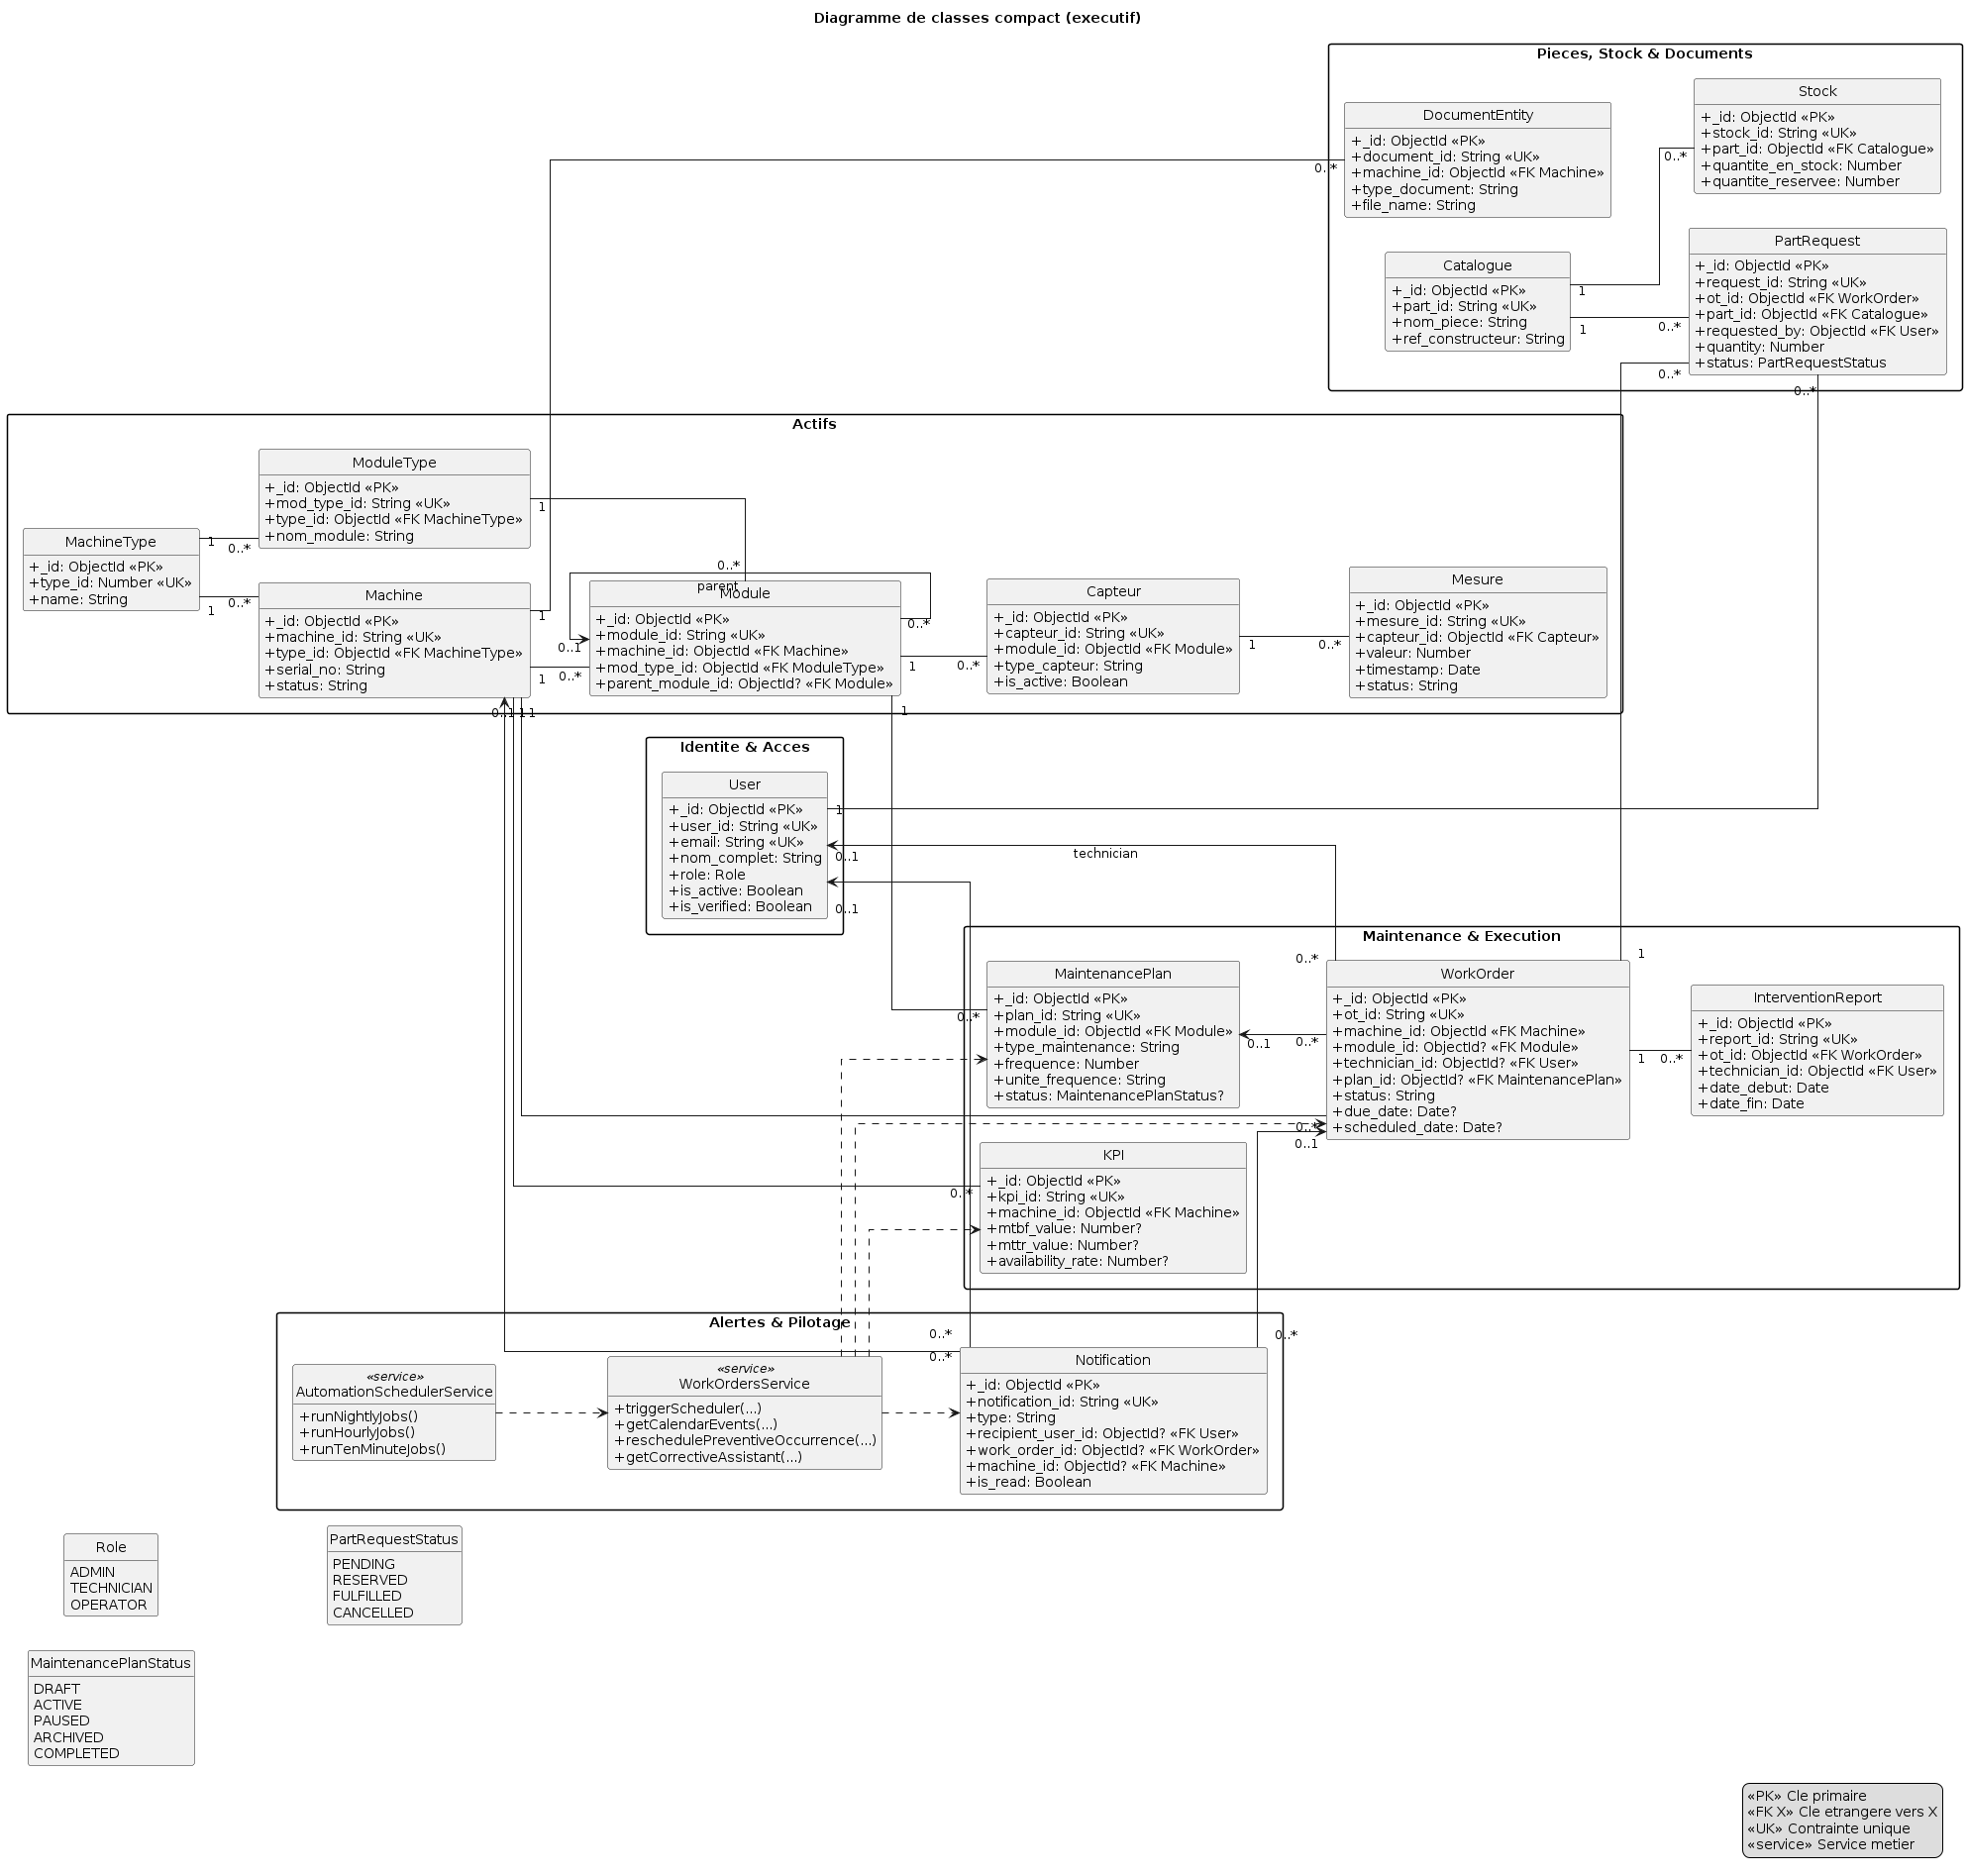
\includegraphics[width=\textwidth]{figures/class-diagram.png}
\caption{Diagramme de classes de la plateforme}
\label{fig:class-diagram}
\end{figure}

Le diagramme met en évidence les principales entités composant le système ainsi que les relations qui existent entre elles.

La classe \textbf{Utilisateur} représente les différents acteurs de la plateforme. Selon le rôle attribué, un utilisateur peut correspondre à un administrateur, un technicien ou un opérateur. Cette classe centralise les informations d'authentification, les données personnelles ainsi que les autorisations d'accès au système.

Les équipements industriels sont modélisés par les classes \textbf{Machine}, \textbf{MachineType}, \textbf{Module} et \textbf{ModuleType}. Cette organisation permet de décrire précisément les caractéristiques techniques des machines ainsi que leur décomposition en différents modules.

Les activités de maintenance sont représentées principalement par les classes \textbf{WorkOrder} et \textbf{InterventionReport}. Les ordres de travail assurent la planification et le suivi des opérations de maintenance préventive ou corrective, tandis que les rapports d'intervention conservent les informations relatives aux opérations effectivement réalisées sur les équipements.

La gestion documentaire est assurée par la classe \textbf{Document}, qui permet d'associer des manuels techniques et des documents PDF aux différentes machines afin de faciliter les interventions des techniciens et des opérateurs.

Le système intègre également plusieurs classes complémentaires destinées à la gestion des pièces de rechange, des catalogues, des indicateurs de performance ainsi que des données nécessaires au fonctionnement global de la plateforme.

Cette organisation modulaire favorise la réutilisabilité des composants, facilite les évolutions futures de l'application et améliore la maintenabilité de l'ensemble du système.
L'implémentation de la plateforme repose sur une base de données orientée documents (MongoDB). Par conséquent, certaines associations représentées dans le diagramme de classes sont matérialisées au niveau de la base de données par des références entre documents plutôt que par des relations relationnelles classiques. Le diagramme UML conserve néanmoins son intérêt puisqu'il décrit la structure conceptuelle du système indépendamment du mécanisme de stockage utilisé.
\cite{sommerville2016,pressman2020,fowler2003} 

\fi

\subsection{Environnement de développement}

Le développement, les tests et le déploiement de la plateforme ont nécessité un environnement matériel et logiciel adapté aux technologies utilisées.

\subsubsection{Environnement matériel}

Le développement a été réalisé sur un ordinateur portable dont les principales caractéristiques sont présentées dans le tableau~\ref{tab:environnement-materiel}.

\begin{table}[H]
\centering
\caption{Environnement matériel}
\label{tab:environnement-materiel}
\small
\begin{tabularx}{0.85\textwidth}{|p{4cm}|X|}
\hline
\textbf{Caractéristique} & \textbf{Valeur} \\
\hline
Processeur & \textit{À compléter} \\
\hline
Mémoire vive & \textit{À compléter} \\
\hline
Stockage & \textit{À compléter} \\
\hline
Système d’exploitation & Windows 10 \\
\hline
\end{tabularx}
\end{table}

\subsubsection{Environnement logiciel}

Le tableau~\ref{tab:environnement-logiciel} présente les principaux outils utilisés au cours du projet.

\begin{table}[H]
\centering
\caption{Environnement logiciel}
\label{tab:environnement-logiciel}
\small
\begin{tabularx}{\textwidth}{|p{3.8cm}|X|}
\hline
\textbf{Outil} & \textbf{Rôle dans le projet} \\
\hline
Visual Studio Code & Développement et organisation du code source \\
\hline
Node.js et npm & Exécution et gestion des dépendances du frontend et du backend \\
\hline
Python & Exécution du service FastAPI et du modèle de détection d’anomalies \\
\hline
Git et GitHub & Gestion des versions, hébergement du dépôt et automatisation des workflows \\
\hline
Postman & Vérification manuelle des API REST \\
\hline
PlantUML & Conception et maintenance des diagrammes UML du projet \\
\hline
MongoDB Atlas & Hébergement de la base de données \\
\hline
Supabase Storage & Stockage des documents de la plateforme \\
\hline
Vercel & Déploiement de l’application Next.js \\
\hline
Render & Déploiement de l’API NestJS, du service FastAPI et des outils de supervision \\
\hline
SonarCloud & Analyse statique et suivi de la qualité du code \\
\hline
Prometheus et Grafana & Collecte et visualisation des métriques techniques \\
\hline
Overleaf & Rédaction et mise en forme du rapport \\
\hline
\end{tabularx}
\end{table}

\subsection*{Conclusion}
\addcontentsline{toc}{subsection}{Conclusion}

Ce chapitre a permis de définir le périmètre de la plateforme GMAO, d’identifier ses acteurs et de préciser ses besoins fonctionnels et non fonctionnels. Le diagramme global des cas d’utilisation a synthétisé les interactions entre les utilisateurs, les équipements connectés et les services externes.

Le Product Backlog et la planification des Sprints ont ensuite organisé les fonctionnalités selon leur priorité et leurs dépendances. Enfin, l’architecture générale, le modèle de données et l’environnement technologique ont établi les bases nécessaires à la réalisation de la solution.

Le chapitre suivant sera consacré au Sprint 1, portant sur l’authentification, la gestion des utilisateurs et le contrôle des accès.

\iffalse

Plusieurs outils de développement ont été utilisés afin de faciliter la conception, le développement, le test ainsi que le déploiement de la plateforme.

\begin{table}[H]
\centering
\renewcommand{\arraystretch}{1.3}

\begin{tabular}{|l|p{8cm}|}

\hline

\textbf{Outil} & \textbf{Rôle}

\\

\hline

Visual Studio Code &
Développement de l'application

\\

\hline

Git &
Gestion des versions

\\

\hline

GitHub &
Hébergement du dépôt source

\\

\hline

MongoDB Atlas &
Base de données Cloud

\\

\hline

Postman &
Tests des API REST

\\

\hline

Vercel &
Déploiement du Frontend

\\

\hline

Render &
Déploiement du Backend

\\

\hline

Draw.io &
Conception des diagrammes UML

\\

\hline

Figma &
Conception des maquettes graphiques

\\

\hline

Overleaf &
Rédaction du rapport

\\

\hline

\end{tabular}

\caption{Environnement logiciel}

\label{tab:logiciel}

\end{table}

\subsection{Conclusion}

\addcontentsline{toc}{subsection}{Conclusion}

Dans ce chapitre, nous avons mené une analyse approfondie des besoins relatifs à la plateforme de gestion de la maintenance industrielle développée pour IPROTEX Tunisie. Cette étape a permis d'identifier les différents acteurs du système ainsi que leurs interactions avec la plateforme, tout en mettant en évidence les fonctionnalités essentielles et les exigences non fonctionnelles nécessaires à son bon fonctionnement.

Nous avons ensuite présenté une modélisation fonctionnelle de la solution à travers le diagramme global des cas d'utilisation et la description textuelle des principaux scénarios d'utilisation. Le Product Backlog a également permis de structurer les fonctionnalités selon leur priorité et leur valeur métier, conformément à l'approche Agile Scrum adoptée pour le développement du projet.

Par ailleurs, le diagramme de classes a permis de définir la structure conceptuelle du système, tandis que la présentation de l'environnement de développement et de l'architecture générale a mis en évidence les principaux choix technologiques retenus pour garantir une solution performante, sécurisée, évolutive et adaptée aux besoins de l'entreprise.

L'ensemble de ces éléments constitue une base solide pour la conception et la réalisation de la plateforme. Le chapitre suivant sera consacré à la conception détaillée de la solution, dans lequel seront présentés les principaux diagrammes UML, l'organisation des composants logiciels ainsi que les choix de conception retenus avant leur implémentation.

\fi

\section{Sprint 1 : Gestion de l'inscription et de
l'authentification}

\subsection{Introduction Sprint 1
}
\subsection{Objectif du Sprint}

\subsection{Analyse du sprint 1}

\subsubsection{Sprint Backlog}

\subsubsection{Diagramme des cas d'utilisation Gestion de l'inscription et de
l'authentification}

\textbf{Description textuelle des cas d'utilisation}

\subsubsection{Diagramme de séquence objet du sprint 1}


\subsection{Réalisation}

\textbf{Conclusion}

\section{Sprint 2 : Gestion des utilisateurs et profil
utilisateur}

\subsection{Introduction}

\subsection{Objectif du Sprint}

\subsection{Analyse du sprint 2}

\subsubsection{Diagramme des cas d'utilisation du sprint 2 Gestion Utilisateurs}

\textbf{Description textuelle des cas d'utilisation Gestion Utilisateurs}

\subsubsection{Diagramme des cas d'utilisation du sprint 2 Gestion Profile}

\textbf{Description textuelle des cas d'utilisation Gestion Profile}

\subsubsection{Diagramme de séquence objet du sprint 2}

\textbf{Diagramme de séquence objet Gestion Des utilisateurs}

\textbf{Diagramme de séquence objet Gestion Des profiles }

\subsection{Réalisation}

\textbf{Conclusion}




